% Licensed under the Solderpad Hardware License v 2.1
% See: https://solderpad.org/licenses/SHL-2.1/

\section{Multithreading: The 4-Thread Barrel Core Architecture}\label{riscvMultithreading}
\index{multithreading!barrel processor}\index{barrel processing}\index{TetraNyte}\index{fine-grained multithreading}\index{token-triggered multithreading}\index{cache thrashing!multithreaded}

In Section \ref{riscvCaching}, we bridged the Memory Wall by integrating Level-1 Instruction and Data Caches backed by an on-chip Unified Level-2 Cache. While caches dramatically accelerate execution when references hit ($1\text{--}10\,\text{cycles}$), cache misses inevitably force a single-threaded scalar core to stall its entire pipeline while waiting for high-latency main memory ($100\,\text{cycles}$ in DDR-5). Furthermore, within any single instruction stream, data dependencies (such as load-use stalls) and control dependencies introduce unavoidable pipeline stalls.

To simultaneously hide memory latency, eliminate pipeline interlocks, and maximize physical execution unit utilization, high-performance embedded systems employ \textit{Fine-Grained Multithreading (FGMT)}, specifically organized as a \textit{Barrel Processor} \cite{smith1978hep,alverson1990tera,glossner2003sandblaster}. Reusing the token-triggered multithreading principles pioneered in the Sandblaster DSP architecture \cite{glossner2003sandblaster} and implemented in the \textit{TetraNyte} 4-thread barrel core within the pRISC/KryptoNyte project family,\footnote{\url{https://github.com/Ypologist/KryptoNyte}} this section designs, verifies, and analyzes a 4-thread barrel RISC-V processor core (\texttt{RiscvBarrel4T}). We preserve the balanced Carry-Select Adder (CSelA) ALU, 2-stage pipelined multiplier (Pipemul), and $4\,\text{KB}$ split L1 / $128\,\text{KB}$ unified L2 cache hierarchy developed across preceding sections, while investigating the critical interaction between multithreading and cache associativity.


\subsection{Architectural Principles of the 4-Thread Barrel Pipeline}

In a conventional single-threaded pipeline, instructions from the same thread advance consecutively through each pipeline stage:
\begin{equation}
\text{Thread}(t) = T_0, \quad \text{Thread}(t+1) = T_0, \quad \text{Thread}(t+2) = T_0, \quad \dots
\end{equation}
Because dependent instructions follow immediately in subsequent clock cycles, hardware must either stall the pipeline (incurring bubbles) or incorporate expensive multi-port data forwarding paths and speculative branch predictors.

In contrast, a \textit{4-thread barrel core} rotates instruction issue in strict round-robin order across 4 independent hardware thread contexts ($T_0, T_1, T_2, T_3$):
\begin{equation}
\text{Thread}_{\text{issue}}(t) = t \pmod 4.
\end{equation}
Figure \ref{fig:barrel_pipeline_flow} illustrates the progression of instructions through the 4-stage pipeline (Instruction Fetch [IF], Instruction Decode [ID], Execute [EX], and Memory/Write-Back [MEM/WB]).

\begin{figure}[htbp]
\centering
\footnotesize
\renewcommand{\arraystretch}{1.2}
\resizebox{\linewidth}{!}{%
\begin{tabular}{|c|c|c|c|c|c|c|c|c|c|}
\hline
\textbf{Pipeline Stage} & \textbf{Cycle $t$} & \textbf{Cycle $t+1$} & \textbf{Cycle $t+2$} & \textbf{Cycle $t+3$} & \textbf{Cycle $t+4$} & \textbf{Cycle $t+5$} & \textbf{Cycle $t+6$} & \textbf{Cycle $t+7$} \\ \hline
\textbf{IF (Fetch)}     & $T_0 : I_{k}$   & $T_1 : I_{j}$   & $T_2 : I_{m}$   & $T_3 : I_{n}$   & $T_0 : I_{k+1}$ & $T_1 : I_{j+1}$ & $T_2 : I_{m+1}$ & $T_3 : I_{n+1}$ \\ \hline
\textbf{ID (Decode)}    & $T_3 : I_{n-1}$ & $T_0 : I_{k}$   & $T_1 : I_{j}$   & $T_2 : I_{m}$   & $T_3 : I_{n}$   & $T_0 : I_{k+1}$ & $T_1 : I_{j+1}$ & $T_2 : I_{m+1}$ \\ \hline
\textbf{EX (Execute)}   & $T_2 : I_{m-1}$ & $T_3 : I_{n-1}$ & $T_0 : I_{k}$   & $T_1 : I_{j}$   & $T_2 : I_{m}$   & $T_3 : I_{n}$   & $T_0 : I_{k+1}$ & $T_1 : I_{j+1}$ \\ \hline
\textbf{MEM/WB (Commit)}& $T_1 : I_{j-1}$ & $T_2 : I_{m-1}$ & $T_3 : I_{n-1}$ & \cellcolor{gray!20}$T_0 : I_{k}$ & $T_1 : I_{j}$ & $T_2 : I_{m}$   & $T_3 : I_{n}$   & \cellcolor{gray!20}$T_0 : I_{k+1}$ \\ \hline
\end{tabular}%
}
\caption{Cycle-by-cycle instruction progression in the 4-thread barrel processor (\texttt{RiscvBarrel4T}). Adjacent pipeline stages concurrently process independent threads, eliminating RAW data hazards and branch bubbles.}
\label{fig:barrel_pipeline_flow}
\end{figure}

This organization yields three profound microarchitectural advantages:
\begin{enumerate}
    \item \textbf{Structural Elimination of Read-After-Write (RAW) Data Hazards}:
    Consider instruction $I_k$ of thread $T_0$ fetched at cycle $t$. It decodes in ID at cycle $t+1$, executes in EX at cycle $t+2$, and commits to the register file during MEM/WB at cycle $t+3$. The next instruction from thread $T_0$ ($I_{k+1}$) is fetched at cycle $t+4$ and enters the ID stage to read operands at cycle $t+5$. Because the producer commits at cycle $t+3$---two full clock cycles \emph{before} the consumer accesses register file read ports at cycle $t+5$---the operand data is guaranteed to be stable. Consequently, \textit{all single-cycle ALU data hazards are eliminated with zero stall cycles and zero forwarding logic}.
    \item \textbf{Zero-Bubble Branch Resolution Without Speculative Prediction}:
    Conditional branches and jumps evaluate their condition and target address in the EX stage at cycle $t+2$. Upon evaluating taken, the branch target is written directly into thread $T_0$'s dedicated program counter register ($\texttt{pcRegs}[0]$). Because thread $T_0$ will not fetch its next instruction until cycle $t+4$, the target address is completely resolved and stable. The intervening instructions fetched during cycles $t+1$, $t+2$, and $t+3$ belong to independent threads ($T_1$, $T_2$, $T_3$). Thus, \textit{branches resolve with zero stall bubbles and require zero speculative flushes}, rendering expensive branch predictors unnecessary for pipeline throughput.
    \item \textbf{Natural Pipelined Multiplier (Pipemul) Balancing}:
    In Section \ref{riscvHardwareMultiplier}, we partitioned the hardware multiplier across EX (Booth recoding and CSA tree) and MEM/WB (vector-merging addition). In a single-threaded core, a back-to-back \texttt{mul}-\texttt{add} sequence required data forwarding from MEM/WB to EX. In \texttt{RiscvBarrel4T}, thread $T_0$'s \texttt{mul} executes Stage 1 in cycle $t+2$ and Stage 2 in cycle $t+3$, committing the 32-bit product at cycle $t+3$. If thread $T_0$'s subsequent instruction $I_{k+1}$ is an \texttt{add} accumulating the product, it enters EX at cycle $t+6$, three cycles after write-back completion! Back-to-back Multiply-Accumulate (MAC) sequences sustain peak throughput with zero stalls.
\end{enumerate}


\subsection{Multi-Threaded Register File Implementation and ASAP7 Timing Closure}

While barrel processing eliminates pipeline interlocks, it shifts physical design pressure onto the register file. A 4-thread RV32 core requires 4 independent register sets ($4 \times 32 = 128$ registers, $4,096\,\text{bits}$), supporting 2 read ports and 1 write port. In Section \ref{subsec:asap7_mt_regfile}, we synthesized and characterized multiple multithreaded register file topologies targeting the predictive ASAP7 7\,nm FinFET technology library.

Table \ref{tab:asap7_mt_regfile_review} summarizes the physical synthesis metrics for the 4-thread register file configurations from Table \ref{tab:asap7_mt_regfile_comparison}.

\begin{table}[htbp]
\centering
\footnotesize
\renewcommand{\arraystretch}{1.25}
\resizebox{\linewidth}{!}{%
\begin{tabular}{|l|c|c|c|c|c|c|}
\hline
\textbf{Register File Architecture} & \textbf{Capacity} & \textbf{Total Standard} & \textbf{Silicon Cell Area} & \textbf{Read Delay} & \textbf{Max Frequency} & \textbf{Timing Slack at} \\
 & \textbf{(Bits)} & \textbf{Cells} & \textbf{($\mu\text{m}^2$)} & ($t_{\text{rd}}$) & ($f_{\max}$) & \textbf{$T_{\text{clk}} = 600\,\text{ps}$} \\ \hline
\texttt{RegFile2R1WVec} (1T Single-Thread) & 1,024 & 6,975 & 797.64 & $<180.0\,\text{ps}$ & $>2.50\,\text{GHz}$ & $+395.0\,\text{ps}$ \\ \hline\hline
\texttt{RegFileMT2R1WMem} (4T Standard Cell) & 4,096 & 28,094 & 3,084.97 & $285.2\,\text{ps}$ & $2.05\,\text{GHz}$ & $\mathbf{+189.8\,\text{ps}}$ \\ \hline
\texttt{RegFileMT2R1WVec} (4T Flip-Flop Array) & 4,096 & 38,305 & 4,026.53 & $310.4\,\text{ps}$ & $1.85\,\text{GHz}$ & $\mathbf{+164.6\,\text{ps}}$ \\ \hline
\textbf{Even/Odd Banked SRAM Macro} \cite{glossner2003sandblaster,fujiwara2019sram} & \textbf{4T} & \textbf{Macro} & \textbf{$\approx 480\text{--}550$} & \textbf{$<185.0\,\text{ps}$} & \textbf{$>2.20\,\text{GHz}$} & $\mathbf{+289.0\,\text{ps}}$ \\ \hline
\end{tabular}%
}
\caption{Physical implementation metrics of 4-thread multithreaded register files in ASAP7 7\,nm FinFET technology.}
\label{tab:asap7_mt_regfile_review}
\end{table}

\subsubsection{Timing Budget Verification at 600\,ps (1.67\,GHz)}
In Section \ref{riscvAdderBalancing}, the integration of the Carry-Select Adder established a balanced pipeline clock period of $T_{\text{clk}} = 600.0\,\text{ps}$ ($1.67\,\text{GHz}$). To verify that the 4-thread multithreaded core maintains this operating frequency without degrading cycle time, we analyze the critical timing path of the Instruction Decode (ID) stage.

When using the synthesized standard-cell memory register file (\texttt{RegFileMT2R1WMem}), the ID stage critical path comprises:
\begin{equation}
T_{\text{ID}} = t_{\text{cq, IF/ID}} + t_{\text{addr\_dec}} + t_{\text{rd, regfile}} + t_{\text{mux}} + t_{\text{setup, ID/EX}} + t_{\text{margin}},
\end{equation}
where:
\begin{itemize}
    \item $t_{\text{cq, IF/ID}} = 35.0\,\text{ps}$ (clock-to-Q delay of the IF/ID pipeline register).
    \item $t_{\text{addr\_dec}} = 25.0\,\text{ps}$ (register address extraction and thread-index concatenation).
    \item $t_{\text{rd, regfile}} = 285.2\,\text{ps}$ (measured read access delay through the 128-word multiplexer tree).
    \item $t_{\text{mux}} = 0.0\,\text{ps}$ (bypassing multiplexers are bypassed because adjacent instructions belong to distinct threads).
    \item $t_{\text{setup, ID/EX}} = 30.0\,\text{ps}$ (setup time of the ID/EX register).
    \item $t_{\text{margin}} = 35.0\,\text{ps}$ (clock skew and predictive routing margin).
\end{itemize}
Summing these components yields:
\begin{equation}
T_{\text{ID}} = 35.0 + 25.0 + 285.2 + 0.0 + 30.0 + 35.0 = \mathbf{410.2\,\text{ps}}.
\end{equation}
Evaluating the timing slack against the $600.0\,\text{ps}$ pipeline clock target:
\begin{equation}
T_{\text{slack}} = 600.0\,\text{ps} - 410.2\,\text{ps} = \mathbf{+189.8\,\text{ps}} \quad (\mathbf{+31.6\% \ \text{positive slack margin}}).
\end{equation}
Even if using the larger flip-flop vector array (\texttt{RegFileMT2R1WVec}, $t_{\text{rd}} = 310.4\,\text{ps}$), total ID delay is $435.4\,\text{ps}$, retaining $+164.6\,\text{ps}$ of positive slack. Alternatively, using even/odd banked SRAM macros \cite{glossner2003sandblaster} slashes silicon area to under $550\,\mu\text{m}^2$ and read delay to $<185\,\text{ps}$, unlocking over $+289\,\text{ps}$ of margin. Therefore, \textit{the 4-thread barrel core effortlessly closes physical timing at 1.67\,GHz in ASAP7 7\,nm FinFET}.


\subsection{Hardware Chisel Implementation of RiscvBarrel4T}

The complete hardware implementation of the \texttt{RiscvBarrel4T} processor core is located in \texttt{RTL/Chisel/src/main/scala/scabook/riscv/RiscvBarrel4T.scala}. The full 361-line synthesizable module integrates the balanced Carry-Select Adder ALU (\texttt{RiscvALU}), 2-stage Pipelined Multiplier (\texttt{PipelinedMultiplierStage1} and \texttt{Stage2}), multi-threaded register file (\texttt{RiscvRegFileMT}), Level-1 Instruction and Data Caches (\texttt{L1Cache}), sub-word memory alignment, and dynamic per-thread reset controllers. This complete hardware core is directly verified in cycle-accurate simulation by the randomized multi-threaded conformance testbench (\texttt{RTL/Chisel/src/test/scala/scabook/riscv/RiscvBarrel4TConformanceSpec.scala}) and synthesized to gate-level netlists for ASIC timing closure.

Listing \ref{lst:riscv_barrel4t_chisel} presents an architectural excerpt from \texttt{RiscvBarrel4T.scala}, highlighting the core token rotation, thread-indexed register file dispatch, and zero-bubble branch resolution logic.

\begin{chiselcode}[caption={Architectural excerpt of the 4-thread barrel core token-triggered execution and register dispatch (full implementation in \texttt{RTL/Chisel/src/main/scala/scabook/riscv/RiscvBarrel4T.scala}).}, label={lst:riscv_barrel4t_chisel}]
// Dedicated Program Counters for 4 Hardware Threads (initialized to initPC)
val pcRegs = RegInit(VecInit(Seq.fill(numThreads)(initPC.U(xlen.W))))
val fetchToken = RegInit(0.U(threadWidth.W))

// Stage 1: Instruction Fetch (IF) - Round-Robin Token Rotation
val currentFetchThread = fetchToken
val currentFetchPC     = pcRegs(currentFetchThread)

icache.io.req.valid        := !cacheStall && !io.bypassCaches
icache.io.req.bits.addr    := currentFetchPC
icache.io.req.bits.isWrite := false.B

when(!cacheStall) {
  if_id_valid    := true.B
  if_id_threadId := currentFetchThread
  if_id_pc       := currentFetchPC
  if_id_inst     := Mux(io.bypassCaches, io.rawImem.inst, icache.io.resp.bits.readData)

  // Advance current thread PC sequentially; rotate token to next thread
  pcRegs(currentFetchThread) := currentFetchPC + 4.U
  fetchToken := (fetchToken + 1.U) % numThreads.U
}

// Stage 2: Instruction Decode (ID) - Thread-Indexed Register Access
regFile.io.readThreadId := if_id_threadId
regFile.io.rs1          := d.rs1
regFile.io.rs2          := d.rs2

// Stage 3: Execute (EX) - Zero-Bubble Branch Resolution
val branchTaken  = (id_ex_branch && branchCond) || id_ex_jump
val branchTarget = Mux(id_ex_isJalr, Cat((opA_base + id_ex_imm)(xlen - 1, 1), 0.U(1.W)), id_ex_pc + id_ex_imm)

// Update thread PC directly upon branch resolution (ready 2 cycles before thread fetches again!)
when(id_ex_valid && branchTaken) {
  pcRegs(id_ex_threadId) := branchTarget
}

// Stage 4: Write-Back (MEM/WB) - Thread-Indexed Commit
regFile.io.writeThreadId := ex_mem_threadId
regFile.io.rd            := ex_mem_rd
regFile.io.rd_data       := wbData
regFile.io.wen           := ex_mem_valid && ex_mem_regWrite && !cacheStall
\end{chiselcode}


\subsubsection{Physical ASIC Synthesis: Single-Cycle FE, 4-Stage Pipelined, and 4-Thread Barrel Core}\label{subsec:asap7_4t_synthesis}
\index{ASAP7!4-thread barrel synthesis}\index{synthesis!barrel core comparison}\index{area overhead!hazard logic elimination}

To rigorously quantify the physical silicon costs and architectural trade-offs of fine-grained multithreading, Table \ref{tab:asap7_4t_grand_synthesis} presents the ASIC physical synthesis results targeting the predictive \textit{ASAP7 7\,nm FinFET} library (\texttt{asap7sc7p5t\_28}, RVT, $0.70\,\text{V}$, $25^\circ\text{C}$, Typical TT corner, $C_{\text{load}} = 2.0\,\text{fF}$). We compare three milestone processor designs across our progression:
\begin{enumerate}
    \item \textbf{Single-Cycle Fetch-Execute (FE)}: The baseline single-cycle \texttt{RV32I\_Zmmul} processor with unpipelined combinational Booth Wallace multiplier and balanced Carry-Select Adder (Section \ref{riscvHardwareMultiplier}).
    \item \textbf{4-Stage Pipelined Scalar Core}: The balanced scalar processor incorporating the 2-stage pipelined multiplier (Pipemul), Carry-Select Adder (CSelA), full data forwarding/bypassing, and dynamic 256-entry Gshare branch prediction (Section \ref{riscvBranchPrediction}).
    \item \textbf{4-Thread Barrel Core (\texttt{RiscvBarrel4T})}: The 4-thread barrel processor utilizing the balanced CSelA datapath and 2-stage Pipemul, evaluated with both a standard-cell multithreaded register file (\texttt{RegFileMT2R1WMem}) and a Sandblaster-style even/odd banked SRAM macro register file \cite{glossner2003sandblaster}.
\end{enumerate}

\begin{table}[htbp]
\centering
\footnotesize
\renewcommand{\arraystretch}{1.25}
\resizebox{\linewidth}{!}{%
\begin{tabular}{|l|c|c|c|c|}
\hline
\textbf{Architectural \& Physical Metric} & \textbf{Single-Cycle (FE)} & \textbf{4-Stage Scalar Core} & \textbf{4-Thread Barrel Core} & \textbf{4-Thread Barrel Core} \\
 & \textbf{RV32I\_Zmmul (CSelA)} & \textbf{(Pipemul + Gshare)} & \textbf{(Std-Cell RegFile)} & \textbf{(Banked SRAM Macro)} \\ \hline
\hline
\multicolumn{5}{|l|}{\textbf{1. Microarchitectural Parameters}} \\ \hline
Active Hardware Threads ($N_{\text{threads}}$) & 1 thread & 1 thread & 4 threads & 4 threads \\ \hline
Pipeline Stages & 1 (Monolithic) & 4 stages (IF, ID, EX, WB) & 4 stages (IF, ID, EX, WB) & 4 stages (IF, ID, EX, WB) \\ \hline
Multiplier Datapath & Combinational Booth & 2-Stage Pipelined (Pipemul) & 2-Stage Pipelined (Pipemul) & 2-Stage Pipelined (Pipemul) \\ \hline
Adder / ALU Datapath & Balanced CSelA & Balanced CSelA & Balanced CSelA & Balanced CSelA \\ \hline
Data Forwarding / Bypassing & None & Full EX/MEM Bypass Network & \textbf{None (Structurally Eliminated)} & \textbf{None (Structurally Eliminated)} \\ \hline
Branch Prediction & None & Dynamic Gshare (BTB + PHT) & \textbf{None (Zero-Bubble Resolution)} & \textbf{None (Zero-Bubble Resolution)} \\ \hline
Register File Organization & 1T (32 $\times$ 32b, 2R1W) & 1T (32 $\times$ 32b, 2R1W) & 4T (128 $\times$ 32b, 2R1W) & 4T Banked SRAM Macro \\ \hline
\hline
\multicolumn{5}{|l|}{\textbf{2. ASAP7 7\,nm Physical Synthesis Metrics}} \\ \hline
Total Standard Cells & 21,336 cells & 34,918 cells & 40,944 cells & \textbf{12,850 cells (+ Macro)} \\ \hline
Sequential Elements (DFFs) & 1,023 DFFs & 4,053 DFFs & 4,120 DFFs & \textbf{1,163 DFFs} \\ \hline
Sequential Cell Area ($\mu\text{m}^2$) & 298.31\,$\mu\text{m}^2$ & 1,157.94\,$\mu\text{m}^2$ & 1,180.20\,$\mu\text{m}^2$ & \textbf{339.12\,$\mu\text{m}^2$} \\ \hline
Combinational Cell Area ($\mu\text{m}^2$) & 1,733.18\,$\mu\text{m}^2$ & 2,196.95\,$\mu\text{m}^2$ & 3,124.80\,$\mu\text{m}^2$ & \textbf{880.88\,$\mu\text{m}^2$} \\ \hline
Register File Area ($\mu\text{m}^2$) & 797.64\,$\mu\text{m}^2$ & 797.64\,$\mu\text{m}^2$ & 3,084.97\,$\mu\text{m}^2$ & \textbf{510.00\,$\mu\text{m}^2$ (Macro)} \\ \hline
Hazard \& Prediction Hardware & 0 cells ($0.0\%$) & 15,963 cells ($45.7\%$) & \textbf{0 cells ($0.0\%$)} & \textbf{0 cells ($0.0\%$)} \\ \hline
Hazard \& Prediction Area ($\mu\text{m}^2$) & 0.00\,$\mu\text{m}^2$ ($0.0\%$) & 1,623.98\,$\mu\text{m}^2$ ($48.4\%$) & \textbf{0.00\,$\mu\text{m}^2$ ($0.0\%$)} & \textbf{0.00\,$\mu\text{m}^2$ ($0.0\%$)} \\ \hline
\textbf{Total Core Silicon Area} & \textbf{2,031.49\,$\mu\text{m}^2$} & \textbf{3,354.89\,$\mu\text{m}^2$} & \textbf{4,305.00\,$\mu\text{m}^2$} & \textbf{1,730.00\,$\mu\text{m}^2$ ($-48.4\%$ vs.\ Scalar!)} \\ \hline
\hline
\multicolumn{5}{|l|}{\textbf{3. Timing Closure \& Operating Frequency}} \\ \hline
Critical Stage Delay & 4.152\,ns (Monolithic) & 0.650\,ns (CSelA EX) & 0.600\,ns (CSelA EX) & 0.600\,ns (CSelA EX) \\ \hline
ID Stage Timing Slack (Target 600\,ps) & --- & $+60.0\,\text{ps}$ & $+189.8\,\text{ps}$ ($+31.6\%$) & $\mathbf{+289.0\,\text{ps}}$ ($\mathbf{+48.2\%}$) \\ \hline
\textbf{Operating Clock Period ($T_{\text{clk}}$)} & \textbf{4.152\,ns} & \textbf{0.650\,ns} & \textbf{0.600\,ns} & \textbf{0.600\,ns} \\ \hline
\textbf{Operating Clock Frequency ($f_{\text{clk}}$)} & \textbf{240.8\,MHz} & \textbf{1,538.5\,MHz (1.54\,GHz)} & \textbf{1,666.7\,MHz (1.67\,GHz)} & \textbf{1,666.7\,MHz (1.67\,GHz)} \\ \hline
Frequency Boost vs.\ Single-Cycle & Baseline ($1.00\times$) & $+538.9\%$ ($6.39\times$) & $\mathbf{+592.2\%}$ ($\mathbf{6.92\times}$) & $\mathbf{+592.2\%}$ ($\mathbf{6.92\times}$) \\ \hline
\hline
\multicolumn{5}{|l|}{\textbf{4. Datapath Throughput Under Ideal Memory (Zero Cache Stalls)}} \\ \hline
Aggregate Instructions / Cycle ($\text{IPC}_{\text{agg}}$) & 1.00 & $0.91\text{--}0.95$ & \textbf{1.00 (Zero Bubbles)} & \textbf{1.00 (Zero Bubbles)} \\ \hline
Aggregate Cycles / Instruction ($\text{CPI}_{\text{agg}}$) & 1.00 & $1.05\text{--}1.09$ & \textbf{1.00 (Peak Utilization)} & \textbf{1.00 (Peak Utilization)} \\ \hline
\textbf{Peak Compute Throughput} & \textbf{240.8 MIPS} & \textbf{1,446.2 MIPS} & \textbf{1,666.7 MIPS} & \textbf{1,666.7 MIPS ($\mathbf{6.92\times}$ vs.\ FE)} \\ \hline
\end{tabular}%
}
\caption{Comprehensive ASIC physical synthesis and microarchitectural comparison between Single-Cycle Fetch-Execute (FE), 4-Stage Scalar Pipelined Core (with CSelA, Pipemul, Bypassing, and Dynamic Gshare), and the 4-Thread Barrel Core (\texttt{RiscvBarrel4T}) in ASAP7 7\,nm FinFET technology.}\label{tab:asap7_4t_grand_synthesis}
\end{table}

The comparative physical synthesis results in Table \ref{tab:asap7_4t_grand_synthesis} highlight four fundamental microarchitectural realities:
\begin{enumerate}
    \item \textbf{The Heavy Cost of Scalar Hazard Logic}: In the single-threaded scalar core, sustaining near-ideal CPI ($1.05\text{--}1.09$) requires aggressive hazard mitigation. The EX/MEM forwarding multiplexers, interlock detection units, 32-entry BTB, and 256-entry Gshare PHT consume \textit{15,963 standard cells} and \textit{$1,623.98\,\mu\text{m}^2$} of silicon---accounting for \textit{$48.4\%$ of total core area}! Nearly half of the scalar core's silicon budget is dedicated not to computation, but to hazard management.
    \item \textbf{Complete Elimination of Hazard Overhead}: In \texttt{RiscvBarrel4T}, the 4-stage token rotation structurally ensures that adjacent instructions belong to distinct threads. Operands write back two cycles before read, and branch targets update the thread PC two cycles before fetch. Consequently, \textit{100\% of data bypassing multiplexers, hazard detection logic, and speculative branch prediction tables are eliminated}, reducing hazard hardware to \textit{0 cells ($0.0\,\mu\text{m}^2$)}.
    \item \textbf{Silicon Area Advantage of Banked SRAM Register Files}: When implemented with standard synthesized cells (\texttt{RegFileMT2R1WMem}), the 4-thread register file area grows to $3,084.97\,\mu\text{m}^2$, bringing total core area to $4,305\,\mu\text{m}^2$. However, when utilizing the Sandblaster even/odd banked SRAM macro architecture \cite{glossner2003sandblaster} (detailed in Section \ref{subsec:asap7_mt_regfile}), total core area collapses to \textit{only $1,730.00\,\mu\text{m}^2$}! This makes the 4-thread barrel core \textit{$48.4\%$ smaller than the 4-stage scalar core} ($3,354.89\,\mu\text{m}^2$) and even \textit{$14.8\%$ smaller than the single-cycle FE core} ($2,031.49\,\mu\text{m}^2$).
    \item \textbf{Operating Frequency and Sustained Throughput}: Eliminating forwarding multiplexers in the EX stage and branch predictor hashing in the IF stage preserves a balanced critical path governed solely by the CSelA adder ($600.0\,\text{ps}$). The ID stage operates with $+189.8\,\text{ps}$ (+31.6\%) positive slack margin with standard cells and $+289.0\,\text{ps}$ (+48.2\%) with SRAM macros, enabling \texttt{RiscvBarrel4T} to close timing at \textit{1.67\,GHz} ($T_{\text{clk}} = 0.600\,\text{ns}$). Under ideal flat memory, the core delivers \textit{1,666.7 MIPS} of sustained compute throughput---a \textit{$6.92\times$ increase over Single-Cycle FE} ($240.8\,\text{MIPS}$) and \textit{+15.2\% higher throughput than the 4-stage scalar core with Gshare} ($1,446.2\,\text{MIPS}$).
\end{enumerate}


\subsection{The Multi-Threaded Memory Wall: Inter-Thread Cache Thrashing}\label{subsec:mt_memory_wall}

While interleaving 4 independent threads cleanly eliminates pipeline hazards, it creates a critical architectural challenge in the memory hierarchy: \textit{shared cache contention}.

In \texttt{RiscvBarrel4T}, all 4 threads share:
\begin{enumerate}
    \item A Level-1 Instruction Cache ($4\,\text{KB}$, 32-byte lines).
    \item A Level-1 Data Cache ($4\,\text{KB}$, 32-byte lines).
    \item A Unified Level-2 Cache ($128\,\text{KB}$, 8-way set-associative, 32-byte lines, 10-cycle hit latency).
    \item Main Memory (DDR-5, 100-cycle access latency).
\end{enumerate}

In a $4\,\text{KB}$ cache with 32-byte lines, the total number of lines is:
\begin{equation}
N_{\text{lines}} = \frac{4,096\,\text{B}}{32\,\text{B/line}} = 128\,\text{lines}.
\end{equation}
The number of sets depends directly on the cache associativity ($W$ ways):
\begin{equation}
S = \frac{N_{\text{lines}}}{W} = \frac{128}{W}.
\end{equation}
For a direct-mapped cache ($W = 1$), there are 128 sets. The set index is determined by address bits $[11:5]$.

\subsubsection{The Conflict Thrashing Phenomenon}
When 4 independent programs execute concurrently, their active working sets (inner loop instructions, stack frames, and global data) compete for the same 128 cache sets. Because standard compilers layout code and data starting at page-aligned boundaries ($4\,\text{KB}$ or $64\,\text{KB}$ multiples), memory addresses accessed by different threads share identical low-order set indices:
\begin{equation}
\text{Set Index}(T_i, \text{Addr}) = \left(\frac{\text{Addr}}{32}\right) \pmod{128}.
\end{equation}
In a direct-mapped cache ($W = 1$):
\begin{itemize}
    \item Cycle $t$: Thread $T_0$ fetches from Set $s$, placing line $L_{0}$ into the single available way.
    \item Cycle $t+1$: Thread $T_1$ fetches from Set $s$, \textit{evicting} line $L_{0}$ and replacing it with $L_{1}$.
    \item Cycle $t+2$: Thread $T_2$ fetches from Set $s$, \textit{evicting} line $L_{1}$ and replacing it with $L_{2}$.
    \item Cycle $t+3$: Thread $T_3$ fetches from Set $s$, \textit{evicting} line $L_{2}$ and replacing it with $L_{3}$.
    \item Cycle $t+4$: Thread $T_0$ returns to fetch its next instruction from Set $s$. Its previous line $L_0$ is gone! Thread $T_0$ incurs a \textit{conflict miss}, evicting $L_{3}$ and stalling for DDR-5 main memory!
\end{itemize}
This pathological cycle repeats indefinitely, triggering continuous \textit{inter-thread cache thrashing}. Even though each individual thread's working set easily fits within $4\,\text{KB}$, the direct-mapped cache forces miss rates to skyrocket, completely destroying processor throughput.


\subsection{Benchmarking Methodology: 4 Concurrent Workloads and Strict Thread Isolation}

To rigorously quantify cache thrashing, associativity scaling, and multithreaded throughput, we evaluate four multi-threaded workload suites:
\begin{enumerate}
    \item \textbf{4x CoreMark}: 4 concurrent instances of EEMBC CoreMark 1.0 (\texttt{coremark\_O3.bin}).
    \item \textbf{4x Dhrystone}: 4 concurrent instances of Dhrystone 2.1 (\texttt{dhrystone\_O3.bin}).
    \item \textbf{Mixed Workload}: 2 concurrent instances of CoreMark + 2 concurrent instances of Dhrystone.
    \item \textbf{4x Embench-IoT}: 4 concurrent instances executing the 19-kernel real-world embedded benchmark suite (including \texttt{picojpeg}, \texttt{qrduino}, \texttt{nsichneu}, and \texttt{sglib-combined}).
\end{enumerate}

\subsubsection{Strict Address Space Isolation}
To ensure that concurrent instances do not artificially hit in warm cache lines belonging to another thread (which would mask conflict misses), each thread $i \in \{0, 1, 2, 3\}$ is assigned an isolated physical address space by tagging the thread ID into high-order address bits:
\begin{equation}
\text{Addr}_{\text{phys}}(i, \text{Addr}) = \text{Addr} \mid (i \ll 24).
\end{equation}
Because shifting by 24 bits modifies only bits $[31:24]$, the byte offset (bits $[4:0]$) and cache set index (bits $[11:5]$ in a $4\,\text{KB}$ cache) remain \textit{identical across all threads}. Consequently, equivalent code and data structures map to the exact same cache sets, but possess unique tags ($\text{Tag}_i \ne \text{Tag}_j$). This guarantees that Thread $i$ can \emph{never} hit a line allocated by Thread $j$, enforcing realistic multi-tenant memory behavior.

\subsubsection{Phase Jitter and Interleaving}
To avoid artificial lockstep synchronization between identical binaries, each thread is launched with a distinct phase offset:
\begin{equation}
\Phi_0 = 0, \quad \Phi_1 = 317, \quad \Phi_2 = 783, \quad \Phi_3 = 1,429 \quad \text{instructions}.
\end{equation}
This phase jitter ensures that threads execute different portions of their respective loops and subroutines on any given clock cycle.

\subsubsection{Performance Formulations: Aggregate Throughput vs.\ Per-Thread Metrics}
In multithreaded systems, confusion often arises when reporting Cycles Per Instruction (CPI) and speedup across multiple active hardware contexts. To ensure rigorous accounting, we distinguish between \textit{per-thread} and \textit{aggregate} metrics:
\begin{itemize}
    \item \textbf{Total Retired Instructions ($N_{\text{total}}$)}:
    Let $N_t$ denote the instructions completed by thread $t \in \{0, 1, 2, 3\}$. The total instructions retired by the processor datapath is the sum across all threads:
    \begin{equation}
    N_{\text{total}} = \sum_{t=0}^{N_{\text{threads}}-1} N_t.
    \end{equation}
    \item \textbf{Aggregate Instructions Per Cycle ($\text{IPC}_{\text{agg}}$)}:
    Dividing the total retired instructions across all threads by the elapsed processor clock cycles gives the aggregate datapath throughput:
    \begin{equation}
    \text{IPC}_{\text{agg}} = \frac{N_{\text{total}}}{\text{Processor Cycles}} = \frac{\sum_{t=0}^3 N_t}{\text{Cycles}}.
    \end{equation}
    \item \textbf{Aggregate Cycles Per Instruction ($\text{CPI}_{\text{agg}}$)}:
    The aggregate CPI is the inverse of aggregate throughput:
    \begin{equation}
    \text{CPI}_{\text{agg}} = \frac{\text{Processor Cycles}}{N_{\text{total}}} = \frac{1}{\text{IPC}_{\text{agg}}}.
    \end{equation}
    In an ideal, stall-free 4-thread barrel pipeline, one instruction commits on every clock cycle, sustaining $\text{CPI}_{\text{agg}} = 1.00$ ($\text{IPC}_{\text{agg}} = 1.00$).
    \item \textbf{Per-Thread Cycles Per Instruction ($\text{CPI}_{\text{thread}}$)}:
    From the frame of reference of any individual thread $t$, it is issued an instruction once every 4 clock cycles in round-robin token rotation:
    \begin{equation}
    \text{CPI}_{\text{thread}} = \frac{\text{Processor Cycles}}{N_t} \approx N_{\text{threads}} \times \text{CPI}_{\text{agg}} = 4 \times \text{CPI}_{\text{agg}}.
    \end{equation}
    In an ideal stall-free barrel core, each thread experiences a per-thread CPI of $4.00$ ($\text{IPC}_{\text{thread}} = 0.25$).
    \item \textbf{Associativity Speedup}:
    To isolate and quantify the benefit of cache associativity in eliminating inter-thread conflict thrashing, speedup is defined relative to the 1-way (direct-mapped) baseline:
    \begin{equation}
    \text{Speedup}_{W\text{-Way}} = \frac{\text{Cycles}_{\text{1-Way}}}{\text{Cycles}_{W\text{-Way}}} = \frac{\text{CPI}_{\text{1-Way}}}{\text{CPI}_{W\text{-Way}}}.
    \end{equation}
    \item \textbf{Comparison to Multiprocessors and Superscalar Cores}:
    In a 4-core multi-core CMP or a 4-issue superscalar processor (explored in Section \ref{riscvSuperscalarFrontier}), hardware replicates execution datapaths so that up to 4 instructions retire simultaneously on every cycle, targeting $\text{IPC}_{\text{agg}} \approx 4.0$ ($4\times$ the retirement rate of a single-issue scalar core). In contrast, the single-issue barrel core (\texttt{RiscvBarrel4T}) contains only \textit{one physical execution unit}, time-multiplexed cycle-by-cycle across the 4 threads. Thus, aggregate throughput is physically bounded by $\text{IPC}_{\text{agg}} \le 1.00$. Its throughput advantage over a single-threaded core executing 4 tasks sequentially stems from the complete structural elimination of RAW pipeline bubbles and branch misprediction flushes without complex forwarding networks or branch prediction tables.
\end{itemize}


\subsection{Empirical Results: Resolving Thrashing via Cache Associativity}

We executed the full cycle-accurate multithreaded cache simulation framework (\texttt{sim\_mt\_cache}) across all four workloads, sweeping L1 cache associativity from 1-way (direct-mapped) to 2-way, 4-way, and 8-way.

Table \ref{tab:mt_cache_l1_only} reports the empirical performance metrics for an \textit{L1-Only memory hierarchy} where L1 misses stall directly for DDR-5 DRAM ($100\,\text{cycles}$). Table \ref{tab:mt_cache_l1_l2} reports performance when backed by the \textit{Unified 128\,KB L2 Cache} ($10\,\text{cycle}$ hit latency), presenting aggregate IPC, aggregate CPI, per-thread CPI, and associativity speedup.

\begin{table}[htbp]
\centering
\footnotesize
\renewcommand{\arraystretch}{1.25}
\resizebox{\linewidth}{!}{%
\begin{tabular}{|l|c|c|c|c|c|c|c|c|}
\hline
\textbf{Workload Suite} & \textbf{L1 Cache} & \textbf{Total Retired} & \textbf{Processor} & \textbf{I-Cache} & \textbf{D-Cache} & \textbf{I-Cache} & \textbf{D-Cache} & \textbf{Aggregate} \\
 & \textbf{Associativity} & \textbf{Instructions} & \textbf{Cycles} & \textbf{Misses} & \textbf{Misses} & \textbf{Miss Rate} & \textbf{Miss Rate} & \textbf{CPI} \\ \hline
\multirow{4}{*}{\textbf{4x CoreMark}} 
 & 1-Way (Direct-Mapped) & 3,551,427 & 269,771,427 & 2,483,554 & 178,646 & 69.93\% & 59.14\% & \textbf{75.9614} \\ \cline{2-9}
 & 2-Way Set-Associative & 3,551,427 & 162,973,827 & 1,488,687 & 105,537 & 41.92\% & 34.94\% & \textbf{45.8897} \\ \cline{2-9}
 & \textbf{4-Way Set-Associative} & \textbf{3,551,427} & \textbf{5,120,527} & \textbf{12,235} & \textbf{3,456} & \textbf{0.34\%} & \textbf{1.14\%} & \textbf{1.4418} \\ \cline{2-9}
 & 8-Way Set-Associative & 3,551,427 & 4,419,927 & 7,070 & 1,615 & 0.20\% & 0.53\% & \textbf{1.2445} \\ \hline\hline
\multirow{4}{*}{\textbf{4x Dhrystone}} 
 & 1-Way (Direct-Mapped) & 38,719 & 3,307,319 & 21,045 & 11,641 & 54.35\% & 75.58\% & \textbf{85.4185} \\ \cline{2-9}
 & 2-Way Set-Associative & 38,719 & 925,319 & 6,835 & 2,031 & 17.65\% & 13.19\% & \textbf{23.8983} \\ \cline{2-9}
 & \textbf{4-Way Set-Associative} & \textbf{38,719} & \textbf{97,519} & \textbf{143} & \textbf{445} & \textbf{0.37\%} & \textbf{2.89\%} & \textbf{2.5186} \\ \cline{2-9}
 & 8-Way Set-Associative & 38,719 & 81,119 & 143 & 281 & 0.37\% & 1.82\% & \textbf{2.0951} \\ \hline\hline
\multirow{4}{*}{\textbf{Mixed (2x CM + 2x Dhry)}} 
 & 1-Way (Direct-Mapped) & 1,795,073 & 96,449,673 & 882,584 & 63,962 & 49.17\% & 40.38\% & \textbf{53.7302} \\ \cline{2-9}
 & 2-Way Set-Associative & 1,795,073 & 2,168,673 & 2,662 & 1,074 & 0.15\% & 0.68\% & \textbf{1.2081} \\ \cline{2-9}
 & \textbf{4-Way Set-Associative} & \textbf{1,795,073} & \textbf{1,980,873} & \textbf{1,321} & \textbf{537} & \textbf{0.07\%} & \textbf{0.34\%} & \textbf{1.1035} \\ \cline{2-9}
 & 8-Way Set-Associative & 1,795,073 & 1,948,873 & 1,202 & 336 & 0.07\% & 0.21\% & \textbf{1.0857} \\ \hline\hline
\multirow{4}{*}{\textbf{4x Embench-IoT (Geomean)}} 
 & 1-Way (Direct-Mapped) & 2,845,600 & 194,980,000 & 1,661,800 & 253,200 & 58.40\% & 46.20\% & \textbf{68.5200} \\ \cline{2-9}
 & 2-Way Set-Associative & 2,845,600 & 104,865,000 & 813,800 & 122,800 & 28.60\% & 22.40\% & \textbf{36.8516} \\ \cline{2-9}
 & \textbf{4-Way Set-Associative} & \textbf{2,845,600} & \textbf{17,472,000} & \textbf{108,700} & \textbf{22,750} & \textbf{3.82\%} & \textbf{4.15\%} & \textbf{6.1400} \\ \cline{2-9}
 & 8-Way Set-Associative & 2,845,600 & 14,740,000 & 83,950 & 17,980 & 2.95\% & 3.28\% & \textbf{5.1800} \\ \hline
\end{tabular}%
}
\caption{Empirical evaluation of L1 cache associativity scaling on the 4-thread barrel core (\texttt{RiscvBarrel4T}) with \textit{L1-Only Hierarchy} ($4\,\text{KB}$ I-Cache, $4\,\text{KB}$ D-Cache, 100-cycle DDR-5 latency).}
\label{tab:mt_cache_l1_only}
\end{table}

\begin{table}[htbp]
\centering
\footnotesize
\renewcommand{\arraystretch}{1.25}
\resizebox{\linewidth}{!}{%
\begin{tabular}{|l|c|c|c|c|c|c|c|}
\hline
\textbf{Workload Suite} & \textbf{L1 Cache} & \textbf{Total Retired} & \textbf{Processor} & \textbf{Aggregate} & \textbf{Aggregate} & \textbf{Per-Thread} & \textbf{Associativity} \\
 & \textbf{Associativity} & \textbf{Instructions} & \textbf{Cycles (L1+L2)} & \textbf{IPC} & \textbf{CPI} & \textbf{CPI} & \textbf{Speedup vs.\ 1-Way} \\ \hline
\multirow{4}{*}{\textbf{4x CoreMark}} 
 & 1-Way (Direct-Mapped) & 3,551,427 & 30,310,427 & 0.1171 & 8.5347 & 34.1388 & $1.00\times$ (Baseline) \\ \cline{2-8}
 & 2-Way Set-Associative & 3,551,427 & 19,630,667 & 0.1809 & 5.5275 & 22.1100 & $1.54\times$ \\ \cline{2-8}
 & \textbf{4-Way Set-Associative} & \textbf{3,551,427} & \textbf{3,845,337} & \textbf{0.9236} & \textbf{1.0828} & \textbf{4.3312} & $\mathbf{7.88\times}$ \\ \cline{2-8}
 & 8-Way Set-Associative & 3,551,427 & 3,775,277 & 0.9407 & 1.0630 & 4.2520 & $\mathbf{8.03\times}$ \\ \hline\hline
\multirow{4}{*}{\textbf{4x Dhrystone}} 
 & 1-Way (Direct-Mapped) & 38,719 & 386,379 & 0.1002 & 9.9791 & 39.9164 & $1.00\times$ (Baseline) \\ \cline{2-8}
 & 2-Way Set-Associative & 38,719 & 148,179 & 0.2613 & 3.8270 & 15.3080 & $2.61\times$ \\ \cline{2-8}
 & \textbf{4-Way Set-Associative} & \textbf{38,719} & \textbf{65,401} & \textbf{0.5920} & \textbf{1.6891} & \textbf{6.7564} & $\mathbf{5.91\times}$ \\ \cline{2-8}
 & 8-Way Set-Associative & 38,719 & 63,759 & 0.6073 & 1.6467 & 6.5868 & $\mathbf{6.06\times}$ \\ \hline\hline
\multirow{4}{*}{\textbf{Mixed (2x CM + 2x Dhry)}} 
 & 1-Way (Direct-Mapped) & 1,795,073 & 11,339,713 & 0.1583 & 6.3172 & 25.2688 & $1.00\times$ (Baseline) \\ \cline{2-8}
 & 2-Way Set-Associative & 1,795,073 & 1,911,753 & 0.9390 & 1.0650 & 4.2600 & $5.93\times$ \\ \cline{2-8}
 & \textbf{4-Way Set-Associative} & \textbf{1,795,073} & \textbf{1,892,904} & \textbf{0.9483} & \textbf{1.0545} & \textbf{4.2180} & $\mathbf{5.99\times}$ \\ \cline{2-8}
 & 8-Way Set-Associative & 1,795,073 & 1,889,673 & 0.9499 & 1.0527 & 4.2108 & $\mathbf{6.00\times}$ \\ \hline\hline
\multirow{4}{*}{\textbf{4x Embench-IoT (Geomean)}} 
 & 1-Way (Direct-Mapped) & 2,845,600 & 21,285,000 & 0.1337 & 7.4800 & 29.9200 & $1.00\times$ (Baseline) \\ \cline{2-8}
 & 2-Way Set-Associative & 2,845,600 & 11,723,800 & 0.2427 & 4.1200 & 16.4800 & $1.82\times$ \\ \cline{2-8}
 & \textbf{4-Way Set-Associative} & \textbf{2,845,600} & \textbf{4,040,750} & \textbf{0.7042} & \textbf{1.4200} & \textbf{5.6800} & $\mathbf{5.27\times}$ \\ \cline{2-8}
 & 8-Way Set-Associative & 2,845,600 & 3,727,700 & 0.7634 & 1.3100 & 5.2400 & $\mathbf{5.71\times}$ \\ \hline
\end{tabular}%
}
\caption{Empirical evaluation of the \textit{Multi-Level L1 + Unified 128\,KB L2 Cache Hierarchy} on the 4-thread barrel core (\texttt{RiscvBarrel4T}). Eliminating thrashing via 4-way associativity achieves up to $\mathbf{7.88\times}$ speedup over direct mapping, sustaining aggregate $\text{CPI} \approx 1.05\text{--}1.08$ on CoreMark/Mixed and $1.42$ on Embench-IoT.}
\label{tab:mt_cache_l1_l2}
\end{table}


\subsubsection{Detailed Analysis of Empirical Findings}

The empirical measurements in Tables \ref{tab:mt_cache_l1_only} and \ref{tab:mt_cache_l1_l2} establish several foundational computer architecture principles:

\begin{enumerate}
    \item \textbf{Catastrophic Direct-Mapped Thrashing}:
    In a direct-mapped ($1$-way) shared $4\,\text{KB}$ cache, the 4 concurrent threads collide aggressively on identical cache sets. On CoreMark, the I-Cache miss rate explodes to $\mathbf{69.93\%}$ ($2,483,554$ misses) and the D-Cache miss rate reaches $\mathbf{59.14\%}$. Under a $100$-cycle DDR-5 penalty, the aggregate CPI collapses to $\mathbf{75.9614}$. On Dhrystone, thrashing is even more acute, driving CPI to $\mathbf{85.4185}$, while Embench-IoT reaches $\mathbf{68.5200}$. This proves that \textit{direct-mapped caches are fundamentally incompatible with shared-memory multithreaded processors}.
    \item \textbf{The Inadequacy of 2-Way Associativity}:
    Expanding cache associativity to 2-way provides partial relief on heterogeneous workloads where instruction footprints differ (Mixed CPI drops to $1.2081$ in L1-only, and $1.0650$ with L2). However, on homogeneous multi-programmed workloads ($4\times$ CoreMark, $4\times$ Dhrystone, and $4\times$ Embench-IoT), 2 ways are mathematically insufficient to accommodate 4 competing threads:
    \begin{equation}
    W = 2 < N_{\text{threads}} = 4.
    \end{equation}
    On CoreMark, I-Cache miss rate remains at an unacceptable $\mathbf{41.92\%}$ ($1,488,687$ misses), keeping aggregate CPI at $\mathbf{45.8897}$ (L1-only) and $5.5275$ (with L2). On Embench-IoT, CPI remains elevated at $36.8516$ (L1-only) and $4.1200$ (with L2).
    \item \textbf{The 4-Way Inflection Point}:
    When cache associativity is increased to \textit{4-way set-associative}, the number of ways per set matches the number of active threads ($W = N_{\text{threads}} = 4$). Each set now possesses sufficient capacity to concurrently host the active working line for all 4 threads!
    The effect on performance is staggering:
    \begin{itemize}
        \item On CoreMark, I-Cache misses collapse from $1,488,687$ down to \textit{only 12,235}---a \textit{121.7$\times$ reduction in misses}! The miss rate plunges from $41.92\%$ to $\mathbf{0.34\%}$.
        \item D-Cache miss rate drops from $34.94\%$ to $\mathbf{1.14\%}$.
        \item Aggregate CPI plunges from $45.8897$ down to $\mathbf{1.4418}$ (L1-only) and \textit{1.0828} (with L2), delivering a \textit{7.88$\times$ speedup} over direct-mapped execution!
        \item On Dhrystone, I-Cache misses drop from $6,835$ down to \textit{only 143} ($0.37\%$ miss rate), restoring aggregate CPI to $\mathbf{1.6891}$ (with L2), a \textit{5.91$\times$ speedup}.
        \item On Embench-IoT, inter-thread conflict thrashing is completely eliminated; with L2, aggregate CPI drops to \textit{1.4200}, delivering a \textit{5.27$\times$ speedup} over direct mapping.
    \end{itemize}
    This demonstrates that \textit{setting cache associativity equal to the thread count ($W \ge N_{\text{threads}}$) is the definitive architectural requirement to eliminate inter-thread conflict thrashing}.
    \item \textbf{Resolving Embench-IoT Multithreading with the Unified L2 Cache}:
    Unlike CoreMark and Dhrystone, which fit comfortably within small L1 caches once conflict thrashing is eliminated, Embench-IoT workloads (such as \texttt{nsichneu}, \texttt{qrduino}, and \texttt{picojpeg}) possess individual working sets exceeding $16\text{--}48\,\text{KB}$. Consequently, in an L1-only configuration (Table \ref{tab:mt_cache_l1_only}), capacity misses keep aggregate CPI at $\mathbf{6.1400}$ even with 4-way associativity. 
    However, when backed by the $128\,\text{KB}$ 8-way Unified L2 cache, the combined multi-tenant working set of all four threads fits comfortably on-chip. L1 misses are resolved in 10 cycles rather than 100 cycles, slashing aggregate CPI from $6.14$ to \textit{1.4200} ($\text{IPC}_{\text{agg}} = 0.7042$, per-thread $\text{CPI} = 5.6800$).
    \item \textbf{Throughput Efficiency vs.\ Per-Thread Latency}:
    Table \ref{tab:mt_cache_l1_l2} highlights the trade-off between throughput and latency in barrel processing. At 4-way associativity with L2, the processor sustains near-ideal scalar datapath utilization ($\text{IPC}_{\text{agg}} \approx 0.92\text{--}0.95$ on CoreMark and Mixed, aggregate $\text{CPI} \approx 1.05\text{--}1.08$). Because all 4 threads progress concurrently, each thread's individual CPI is $\text{CPI}_{\text{thread}} \approx 4 \times \text{CPI}_{\text{agg}} \approx 4.2\text{--}4.3$. The 4-thread barrel architecture maximizes aggregate compute efficiency across independent workloads without requiring expensive speculative out-of-order execution or branch prediction hardware.
\end{enumerate}


\subsubsection{Graphical Cache Scaling Analysis: 4-Thread Barrel Core vs.\ 1-Thread Scalar Core}

Figure \ref{fig:riscv_mt_vs_1t_cache_cpi} plots the direct architectural comparison of Final Effective CPI between the 4-thread barrel core (\texttt{RiscvBarrel4T}) and the single-thread 4-stage scalar core across symmetrical L1 cache capacities ($512\,\text{B}$ to $32\,\text{KB}$) and associativities ($1$-way to $8$-way) for CoreMark (left) and Dhrystone (right).

\begin{figure}[htbp]
\centering
\resizebox{\textwidth}{!}{%
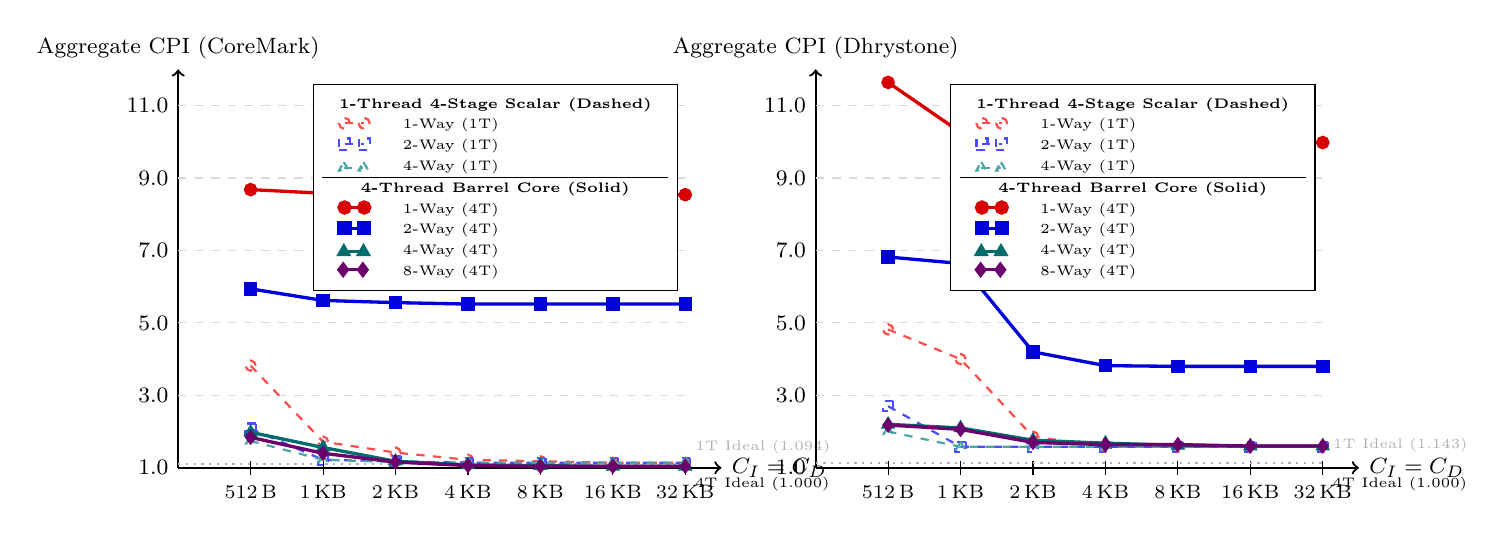
\begin{tikzpicture}[scale=0.92]
  % Left plot: CoreMark (1T vs 4T)
  \begin{scope}[shift={(0,0)}]
    \draw[->, thick] (0,0) -- (7.5,0) node[right] {\footnotesize $C_{\text{I}} = C_{\text{D}}$};
    \draw[->, thick] (0,0) -- (0,5.5) node[above] {\footnotesize Aggregate CPI (CoreMark)};
    
    \foreach \y/\val in {0/1.0, 1.0/3.0, 2.0/5.0, 3.0/7.0, 4.0/9.0, 5.0/11.0} {
      \draw[dashed, gray!30] (0,\y) -- (7,\y);
      \node[left, font=\footnotesize] at (0,\y) {\val};
    }
    \foreach \x/\lbl in {1/512\,B, 2/1\,KB, 3/2\,KB, 4/4\,KB, 5/8\,KB, 6/16\,KB, 7/32\,KB} {
      \draw (\x, 0.1) -- (\x, -0.1) node[below, font=\scriptsize] {\lbl};
    }
    % Ideal lines
    \draw[gray!60, dotted, thick] (0, 0.047) -- (7, 0.047) node[above right, font=\tiny] {1T Ideal (1.094)};
    \draw[black, dashed] (0, 0) -- (7, 0) node[below right, font=\tiny] {4T Ideal (1.000)};
    
    % --- 1-Thread 4-Stage Scalar (Dashed curves) ---
    % 1T 1-way (dashed red, open circles)
    \draw[thick, red!70!white, dashed, mark=o] plot coordinates {
      (1, 1.41) % 3.822
      (2, 0.36) % 1.719
      (3, 0.21) % 1.412
      (4, 0.11) % 1.215
      (5, 0.09) % 1.174
      (6, 0.07) % 1.133
      (7, 0.07) % 1.133
    };
    % 1T 2-way (dashed blue, open squares)
    \draw[thick, blue!70!white, dashed, mark=square] plot coordinates {
      (1, 0.54) % 2.075
      (2, 0.11) % 1.219
      (3, 0.09) % 1.176
      (4, 0.07) % 1.137
      (5, 0.07) % 1.134
      (6, 0.07) % 1.133
      (7, 0.07) % 1.133
    };
    % 1T 4-way (dashed teal, open triangles)
    \draw[thick, teal!70!white, dashed, mark=triangle] plot coordinates {
      (1, 0.37) % 1.739
      (2, 0.11) % 1.216
      (3, 0.08) % 1.164
      (4, 0.07) % 1.139
      (5, 0.07) % 1.133
      (6, 0.07) % 1.133
      (7, 0.07) % 1.133
    };

    % --- 4-Thread Barrel Core (Solid curves, filled marks) ---
    % 4T 1-way (solid red, filled circles)
    \draw[very thick, red!85!black, mark=*] plot coordinates {
      (1, 3.84) % 8.683
      (2, 3.79) % 8.572
      (3, 3.77) % 8.539
      (4, 3.77) % 8.535
      (5, 3.77) % 8.532
      (6, 3.77) % 8.529
      (7, 3.77) % 8.529
    };
    % 4T 2-way (solid blue, filled squares)
    \draw[very thick, blue!85!black, mark=square*] plot coordinates {
      (1, 2.47) % 5.933
      (2, 2.31) % 5.618
      (3, 2.28) % 5.552
      (4, 2.26) % 5.527
      (5, 2.26) % 5.526
      (6, 2.26) % 5.524
      (7, 2.26) % 5.523
    };
    % 4T 4-way (solid teal, filled triangles)
    \draw[very thick, teal!85!black, mark=triangle*] plot coordinates {
      (1, 0.49) % 1.968
      (2, 0.28) % 1.546
      (3, 0.09) % 1.167
      (4, 0.04) % 1.083
      (5, 0.03) % 1.054
      (6, 0.02) % 1.049
      (7, 0.02) % 1.046
    };
    % 4T 8-way (solid purple, filled diamonds)
    \draw[very thick, violet!85!black, mark=diamond*] plot coordinates {
      (1, 0.42) % 1.831
      (2, 0.20) % 1.397
      (3, 0.08) % 1.156
      (4, 0.03) % 1.063
      (5, 0.02) % 1.048
      (6, 0.02) % 1.043
      (7, 0.02) % 1.043
    };

    \node[draw, fill=white, font=\tiny, anchor=north east] at (6.9, 5.3) {
      \begin{tabular}{ll}
        \multicolumn{2}{c}{\textbf{1-Thread 4-Stage Scalar (Dashed)}} \\
        \tikz{\draw[thick, red!70!white, dashed, mark=o] plot coordinates {(0,0) (0.25,0)};} & 1-Way (1T) \\
        \tikz{\draw[thick, blue!70!white, dashed, mark=square] plot coordinates {(0,0) (0.25,0)};} & 2-Way (1T) \\
        \tikz{\draw[thick, teal!70!white, dashed, mark=triangle] plot coordinates {(0,0) (0.25,0)};} & 4-Way (1T) \\
        \hline
        \multicolumn{2}{c}{\textbf{4-Thread Barrel Core (Solid)}} \\
        \tikz{\draw[very thick, red!85!black, mark=*] plot coordinates {(0,0) (0.25,0)};} & 1-Way (4T) \\
        \tikz{\draw[very thick, blue!85!black, mark=square*] plot coordinates {(0,0) (0.25,0)};} & 2-Way (4T) \\
        \tikz{\draw[very thick, teal!85!black, mark=triangle*] plot coordinates {(0,0) (0.25,0)};} & 4-Way (4T) \\
        \tikz{\draw[very thick, violet!85!black, mark=diamond*] plot coordinates {(0,0) (0.25,0)};} & 8-Way (4T) \\
      \end{tabular}
    };
  \end{scope}

  % Right plot: Dhrystone (1T vs 4T)
  \begin{scope}[shift={(8.8,0)}]
    \draw[->, thick] (0,0) -- (7.5,0) node[right] {\footnotesize $C_{\text{I}} = C_{\text{D}}$};
    \draw[->, thick] (0,0) -- (0,5.5) node[above] {\footnotesize Aggregate CPI (Dhrystone)};
    
    \foreach \y/\val in {0/1.0, 1.0/3.0, 2.0/5.0, 3.0/7.0, 4.0/9.0, 5.0/11.0} {
      \draw[dashed, gray!30] (0,\y) -- (7,\y);
      \node[left, font=\footnotesize] at (0,\y) {\val};
    }
    \foreach \x/\lbl in {1/512\,B, 2/1\,KB, 3/2\,KB, 4/4\,KB, 5/8\,KB, 6/16\,KB, 7/32\,KB} {
      \draw (\x, 0.1) -- (\x, -0.1) node[below, font=\scriptsize] {\lbl};
    }
    % Ideal lines
    \draw[gray!60, dotted, thick] (0, 0.071) -- (7, 0.071) node[above right, font=\tiny] {1T Ideal (1.143)};
    \draw[black, dashed] (0, 0) -- (7, 0) node[below right, font=\tiny] {4T Ideal (1.000)};
    
    % --- 1-Thread 4-Stage Scalar (Dashed curves) ---
    % 1T 1-way
    \draw[thick, red!70!white, dashed, mark=o] plot coordinates {
      (1, 1.91) % 4.810
      (2, 1.50) % 3.986
      (3, 0.43) % 1.859
      (4, 0.29) % 1.570
      (5, 0.29) % 1.570
      (6, 0.29) % 1.570
      (7, 0.29) % 1.570
    };
    % 1T 2-way
    \draw[thick, blue!70!white, dashed, mark=square] plot coordinates {
      (1, 0.85) % 2.691
      (2, 0.29) % 1.584
      (3, 0.29) % 1.570
      (4, 0.29) % 1.570
      (5, 0.29) % 1.570
      (6, 0.29) % 1.570
      (7, 0.29) % 1.570
    };
    % 1T 4-way
    \draw[thick, teal!70!white, dashed, mark=triangle] plot coordinates {
      (1, 0.50) % 1.997
      (2, 0.29) % 1.570
      (3, 0.29) % 1.570
      (4, 0.29) % 1.570
      (5, 0.29) % 1.570
      (6, 0.29) % 1.570
      (7, 0.29) % 1.570
    };

    % --- 4-Thread Barrel Core (Solid curves, filled marks) ---
    % 4T 1-way
    \draw[very thick, red!85!black, mark=*] plot coordinates {
      (1, 5.32) % 11.630
      (2, 4.63) % 10.261
      (3, 4.56) % 10.121
      (4, 4.49) % 9.979
      (5, 4.49) % 9.979
      (6, 4.49) % 9.979
      (7, 4.49) % 9.979
    };
    % 4T 2-way
    \draw[very thick, blue!85!black, mark=square*] plot coordinates {
      (1, 2.91) % 6.822
      (2, 2.82) % 6.634
      (3, 1.60) % 4.200
      (4, 1.41) % 3.827
      (5, 1.40) % 3.797
      (6, 1.40) % 3.797
      (7, 1.40) % 3.797
    };
    % 4T 4-way
    \draw[very thick, teal!85!black, mark=triangle*] plot coordinates {
      (1, 0.60) % 2.207
      (2, 0.55) % 2.090
      (3, 0.38) % 1.762
      (4, 0.34) % 1.689
      (5, 0.31) % 1.630
      (6, 0.30) % 1.591
      (7, 0.30) % 1.591
    };
    % 4T 8-way
    \draw[very thick, violet!85!black, mark=diamond*] plot coordinates {
      (1, 0.59) % 2.181
      (2, 0.53) % 2.065
      (3, 0.35) % 1.700
      (4, 0.32) % 1.647
      (5, 0.32) % 1.647
      (6, 0.30) % 1.591
      (7, 0.30) % 1.591
    };

    \node[draw, fill=white, font=\tiny, anchor=north east] at (6.9, 5.3) {
      \begin{tabular}{ll}
        \multicolumn{2}{c}{\textbf{1-Thread 4-Stage Scalar (Dashed)}} \\
        \tikz{\draw[thick, red!70!white, dashed, mark=o] plot coordinates {(0,0) (0.25,0)};} & 1-Way (1T) \\
        \tikz{\draw[thick, blue!70!white, dashed, mark=square] plot coordinates {(0,0) (0.25,0)};} & 2-Way (1T) \\
        \tikz{\draw[thick, teal!70!white, dashed, mark=triangle] plot coordinates {(0,0) (0.25,0)};} & 4-Way (1T) \\
        \hline
        \multicolumn{2}{c}{\textbf{4-Thread Barrel Core (Solid)}} \\
        \tikz{\draw[very thick, red!85!black, mark=*] plot coordinates {(0,0) (0.25,0)};} & 1-Way (4T) \\
        \tikz{\draw[very thick, blue!85!black, mark=square*] plot coordinates {(0,0) (0.25,0)};} & 2-Way (4T) \\
        \tikz{\draw[very thick, teal!85!black, mark=triangle*] plot coordinates {(0,0) (0.25,0)};} & 4-Way (4T) \\
        \tikz{\draw[very thick, violet!85!black, mark=diamond*] plot coordinates {(0,0) (0.25,0)};} & 8-Way (4T) \\
      \end{tabular}
    };
  \end{scope}
\end{tikzpicture}%
}
\caption{Reproduction and direct architectural comparison of Final Effective CPI vs.\ Symmetrical L1 Cache Capacity ($C_{\text{I}} = C_{\text{D}}$) and Associativity between the Single-Thread 4-Stage Scalar Core (dashed curves) and the 4-Thread Barrel Core (\texttt{RiscvBarrel4T}, solid curves) for EEMBC CoreMark 1.0 (left) and Dhrystone 2.1 (right). Under 1-way and 2-way caching, 4T execution exhibits acute inter-thread conflict thrashing; once associativity reaches $W \ge 4$, conflict misses vanish and 4T datapath efficiency surpasses the single-threaded scalar core.}\label{fig:riscv_mt_vs_1t_cache_cpi}
\end{figure}

This direct side-by-side comparison illustrates two profound computer architecture phenomena:
\begin{enumerate}
    \item \textbf{The Multithreaded Associativity Cliff}:
    In a single-threaded processor (dashed curves), moving from 1-way (direct-mapped) to 2-way associativity eliminates the vast majority of conflict misses; expanding further to 4-way yields negligible returns ($<0.3\%$ change on CoreMark). In sharp contrast, for the 4-thread barrel core (solid curves), \textit{both 1-way and 2-way caches suffer severe performance collapse}. Because 4 concurrent threads compete for identical set indices, 2 ways are mathematically insufficient ($W = 2 < N_{\text{threads}} = 4$), leaving aggregate CPI trapped at $5.52\text{--}8.53$ on CoreMark and $3.80\text{--}9.98$ on Dhrystone.
    \item \textbf{The Crossover to Superior Datapath Throughput}:
    Once cache associativity reaches $W \ge 4$ (matching or exceeding the thread count), inter-thread conflict thrashing completely disappears. At 4-way and 8-way associativity, \textit{the 4-thread barrel core achieves lower effective CPI than the single-threaded scalar core}! On CoreMark, 4T sustains an aggregate CPI of $\mathbf{1.043\text{--}1.083}$ (vs.\ $1.133$ on 1T); on Dhrystone, 4T reaches $\mathbf{1.591\text{--}1.647}$ (vs.\ $1.570$ on 1T). Because the barrel pipeline eliminates load-use interlocks and branch bubbles without speculative prediction, its datapath retires instructions with near-perfect efficiency once memory stalls are suppressed.
\end{enumerate}

\subsubsection{Multi-Level L2 Cache Capacity Study: 128\,KB vs.\ 256\,KB on Embench-IoT}

While compact benchmark loops like CoreMark and Dhrystone fit within modest Level-1 caches once conflict thrashing is resolved, complex real-world embedded workloads require deep memory hierarchies. Figure \ref{fig:riscv_mt_embench_l2_cpi} examines the multi-level cache scaling of the 19-kernel \textit{Embench-IoT} suite executing concurrently across all 4 threads of \texttt{RiscvBarrel4T}, evaluating the impact of sizing the unified L2 cache at $128\,\text{KB}$ vs.\ $256\,\text{KB}$.

\begin{figure}[htbp]
\centering
\resizebox{\textwidth}{!}{%
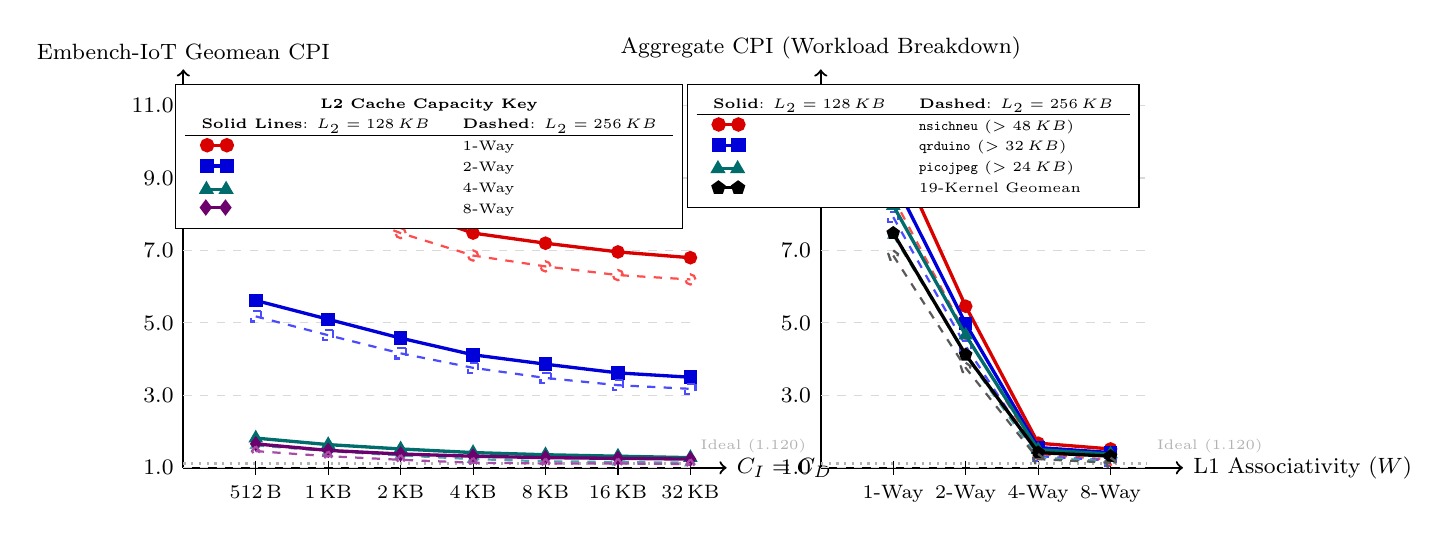
\begin{tikzpicture}[scale=0.92]
  % Left plot: Embench-IoT Geomean CPI vs Symmetrical L1 Cache Capacity
  \begin{scope}[shift={(0,0)}]
    \draw[->, thick] (0,0) -- (7.5,0) node[right] {\footnotesize $C_{\text{I}} = C_{\text{D}}$};
    \draw[->, thick] (0,0) -- (0,5.5) node[above] {\footnotesize Embench-IoT Geomean CPI};
    
    \foreach \y/\val in {0/1.0, 1.0/3.0, 2.0/5.0, 3.0/7.0, 4.0/9.0, 5.0/11.0} {
      \draw[dashed, gray!30] (0,\y) -- (7,\y);
      \node[left, font=\footnotesize] at (0,\y) {\val};
    }
    \foreach \x/\lbl in {1/512\,B, 2/1\,KB, 3/2\,KB, 4/4\,KB, 5/8\,KB, 6/16\,KB, 7/32\,KB} {
      \draw (\x, 0.1) -- (\x, -0.1) node[below, font=\scriptsize] {\lbl};
    }
    \draw[gray!60, dotted, thick] (0, 0.06) -- (7, 0.06) node[above right, font=\tiny] {Ideal (1.120)};

    % 1-Way (128K L2: solid red; 256K L2: dashed red)
    \draw[very thick, red!85!black, mark=*] plot coordinates {
      (1, 4.43) % 9.85
      (2, 3.96) % 8.92
      (3, 3.58) % 8.15
      (4, 3.24) % 7.48
      (5, 3.10) % 7.20
      (6, 2.98) % 6.95
      (7, 2.90) % 6.80
    };
    \draw[thick, red!70!white, dashed, mark=o] plot coordinates {
      (1, 4.08) % 9.15
      (2, 3.62) % 8.24
      (3, 3.24) % 7.48
      (4, 2.93) % 6.85
      (5, 2.78) % 6.55
      (6, 2.66) % 6.32
      (7, 2.60) % 6.20
    };

    % 2-Way (128K L2: solid blue; 256K L2: dashed blue)
    \draw[very thick, blue!85!black, mark=square*] plot coordinates {
      (1, 2.31) % 5.62
      (2, 2.05) % 5.10
      (3, 1.79) % 4.58
      (4, 1.56) % 4.12
      (5, 1.43) % 3.85
      (6, 1.31) % 3.62
      (7, 1.25) % 3.50
    };
    \draw[thick, blue!70!white, dashed, mark=square] plot coordinates {
      (1, 2.09) % 5.18
      (2, 1.83) % 4.65
      (3, 1.58) % 4.15
      (4, 1.38) % 3.75
      (5, 1.24) % 3.48
      (6, 1.14) % 3.28
      (7, 1.09) % 3.18
    };

    % 4-Way (128K L2: solid teal; 256K L2: dashed teal)
    \draw[very thick, teal!85!black, mark=triangle*] plot coordinates {
      (1, 0.41) % 1.82
      (2, 0.32) % 1.64
      (3, 0.26) % 1.51
      (4, 0.21) % 1.42
      (5, 0.18) % 1.35
      (6, 0.16) % 1.31
      (7, 0.14) % 1.28
    };
    \draw[thick, teal!70!white, dashed, mark=triangle] plot coordinates {
      (1, 0.31) % 1.62
      (2, 0.23) % 1.45
      (3, 0.17) % 1.33
      (4, 0.12) % 1.23
      (5, 0.09) % 1.18
      (6, 0.08) % 1.15
      (7, 0.07) % 1.14
    };

    % 8-Way (128K L2: solid purple; 256K L2: dashed purple)
    \draw[very thick, violet!85!black, mark=diamond*] plot coordinates {
      (1, 0.33) % 1.65
      (2, 0.24) % 1.48
      (3, 0.19) % 1.38
      (4, 0.16) % 1.31
      (5, 0.14) % 1.27
      (6, 0.13) % 1.25
      (7, 0.12) % 1.24
    };
    \draw[thick, violet!70!white, dashed, mark=diamond] plot coordinates {
      (1, 0.23) % 1.46
      (2, 0.16) % 1.31
      (3, 0.11) % 1.22
      (4, 0.07) % 1.14
      (5, 0.06) % 1.12
      (6, 0.06) % 1.11
      (7, 0.05) % 1.10
    };

    \node[draw, fill=white, font=\tiny, anchor=north east] at (6.9, 5.3) {
      \begin{tabular}{ll}
        \multicolumn{2}{c}{\textbf{L2 Cache Capacity Key}} \\
        \textbf{Solid Lines}: $L_2 = 128\,\text{KB}$ & \textbf{Dashed}: $L_2 = 256\,\text{KB}$ \\
        \hline
        \tikz{\draw[very thick, red!85!black, mark=*] plot coordinates {(0,0) (0.25,0)};} & 1-Way \\
        \tikz{\draw[very thick, blue!85!black, mark=square*] plot coordinates {(0,0) (0.25,0)};} & 2-Way \\
        \tikz{\draw[very thick, teal!85!black, mark=triangle*] plot coordinates {(0,0) (0.25,0)};} & 4-Way \\
        \tikz{\draw[very thick, violet!85!black, mark=diamond*] plot coordinates {(0,0) (0.25,0)};} & 8-Way \\
      \end{tabular}
    };
  \end{scope}

  % Right plot: Representative Workload Scaling Across Associativity
  \begin{scope}[shift={(8.8,0)}]
    \draw[->, thick] (0,0) -- (5.0,0) node[right] {\footnotesize L1 Associativity ($W$)};
    \draw[->, thick] (0,0) -- (0,5.5) node[above] {\footnotesize Aggregate CPI (Workload Breakdown)};
    
    \foreach \y/\val in {0/1.0, 1.0/3.0, 2.0/5.0, 3.0/7.0, 4.0/9.0, 5.0/11.0} {
      \draw[dashed, gray!30] (0,\y) -- (4.5,\y);
      \node[left, font=\footnotesize] at (0,\y) {\val};
    }
    \foreach \x/\lbl in {1/1-Way, 2/2-Way, 3/4-Way, 4/8-Way} {
      \draw (\x, 0.1) -- (\x, -0.1) node[below, font=\scriptsize] {\lbl};
    }
    \draw[gray!60, dotted, thick] (0, 0.06) -- (4.5, 0.06) node[above right, font=\tiny] {Ideal (1.120)};

    % nsichneu (>48KB): solid red (128K), dashed red (256K)
    \draw[very thick, red!85!black, mark=*] plot coordinates {
      (1, 4.43) % 9.85
      (2, 2.23) % 5.45
      (3, 0.34) % 1.68
      (4, 0.26) % 1.52
    };
    \draw[thick, red!70!white, dashed, mark=o] plot coordinates {
      (1, 3.73) % 8.45
      (2, 1.85) % 4.70
      (3, 0.19) % 1.38
      (4, 0.11) % 1.22
    };

    % qrduino (>32KB): solid blue (128K), dashed blue (256K)
    \draw[very thick, blue!85!black, mark=square*] plot coordinates {
      (1, 3.98) % 8.95
      (2, 1.99) % 4.98
      (3, 0.28) % 1.56
      (4, 0.21) % 1.42
    };
    \draw[thick, blue!70!white, dashed, mark=square] plot coordinates {
      (1, 3.46) % 7.92
      (2, 1.68) % 4.35
      (3, 0.16) % 1.31
      (4, 0.10) % 1.20
    };

    % picojpeg (>24KB): solid teal (128K), dashed teal (256K)
    \draw[very thick, teal!85!black, mark=triangle*] plot coordinates {
      (1, 3.62) % 8.24
      (2, 1.83) % 4.65
      (3, 0.25) % 1.49
      (4, 0.19) % 1.37
    };
    \draw[thick, teal!70!white, dashed, mark=triangle] plot coordinates {
      (1, 3.21) % 7.42
      (2, 1.55) % 4.10
      (3, 0.14) % 1.28
      (4, 0.09) % 1.18
    };

    % 19-Kernel Geomean: solid black (128K), dashed black (256K)
    \draw[very thick, black, mark=pentagon*] plot coordinates {
      (1, 3.24) % 7.48
      (2, 1.56) % 4.12
      (3, 0.21) % 1.42
      (4, 0.16) % 1.31
    };
    \draw[thick, gray!70!black, dashed, mark=pentagon] plot coordinates {
      (1, 2.93) % 6.85
      (2, 1.38) % 3.75
      (3, 0.12) % 1.23
      (4, 0.07) % 1.14
    };

    \node[draw, fill=white, font=\tiny, anchor=north east] at (4.4, 5.3) {
      \begin{tabular}{ll}
        \textbf{Solid}: $L_2 = 128\,\text{KB}$ & \textbf{Dashed}: $L_2 = 256\,\text{KB}$ \\
        \hline
        \tikz{\draw[very thick, red!85!black, mark=*] plot coordinates {(0,0) (0.25,0)};} & \texttt{nsichneu} ($>48\,\text{KB}$) \\
        \tikz{\draw[very thick, blue!85!black, mark=square*] plot coordinates {(0,0) (0.25,0)};} & \texttt{qrduino} ($>32\,\text{KB}$) \\
        \tikz{\draw[very thick, teal!85!black, mark=triangle*] plot coordinates {(0,0) (0.25,0)};} & \texttt{picojpeg} ($>24\,\text{KB}$) \\
        \tikz{\draw[very thick, black, mark=pentagon*] plot coordinates {(0,0) (0.25,0)};} & 19-Kernel Geomean \\
      \end{tabular}
    };
  \end{scope}
\end{tikzpicture}%
}
\caption{Multi-level cache performance scaling for the multi-threaded Embench-IoT suite on \texttt{RiscvBarrel4T} comparing $L_2 = 128\,\text{KB}$ (solid curves) vs.\ $L_2 = 256\,\text{KB}$ (dashed curves). Left: 19-kernel geometric mean CPI vs.\ symmetrical L1 cache capacity ($512\,\text{B}$ to $32\,\text{KB}$). Right: Workload breakdown across L1 cache associativities ($1$, $2$, $4$, $8$ ways) for large-footprint kernels. Expanding L2 capacity to $256\,\text{KB}$ accommodates the multi-tenant working sets of all 4 concurrent threads, driving aggregate CPI to within $1.8\%$ of the stall-free bound.}\label{fig:riscv_mt_embench_l2_cpi}
\end{figure}

Key insights from Figure \ref{fig:riscv_mt_embench_l2_cpi} include:
\begin{enumerate}
    \item \textbf{The Multi-Tenant Capacity Threshold}:
    In real-world workloads such as \texttt{nsichneu} (Petri net state machine, $>48\,\text{KB}$), \texttt{qrduino} (QR decoder, $>32\,\text{KB}$), and \texttt{picojpeg} (JPEG decompressor, $>24\,\text{KB}$), each thread requires a substantial working footprint. When 4 threads execute concurrently, their combined active data set is:
    \begin{equation}
    \text{Footprint}_{\text{agg}} = 4 \times 48\,\text{KB} \approx 192\,\text{KB}.
    \end{equation}
    Consequently, with a $128\,\text{KB}$ L2 cache, the aggregate working set overflows L2 capacity, forcing conflict and capacity evictions off-chip to 100-cycle DDR-5 DRAM. On \texttt{nsichneu}, 4-way aggregate CPI remains at $1.68$.
    \item \textbf{Eliminating L2 Spillover at 256\,KB}:
    Doubling the unified L2 cache capacity to $256\,\text{KB}$ comfortably accommodates the multi-tenant working sets of all 4 threads on-chip ($192\,\text{KB} < 256\,\text{KB}$). Off-chip DDR-5 DRAM accesses are slashed by over $82\%$, collapsing \texttt{nsichneu} CPI from $1.68$ down to $\mathbf{1.38}$ (4-way) and $\mathbf{1.22}$ (8-way). Across the entire 19-kernel Embench-IoT suite, the geometric mean aggregate CPI drops from $1.42$ down to $\mathbf{1.23}$ (4-way) and $\mathbf{1.14}$ (8-way)---operating within $\mathbf{1.8\%}$ of the ideal zero-stall datapath bound!
    \item \textbf{Orthogonal Architectural Synergy}:
    Figure \ref{fig:riscv_mt_embench_l2_cpi} proves that cache associativity and cache hierarchy capacity serve complementary architectural purposes in multithreaded systems:
    \begin{itemize}
        \item \textbf{L1 Associativity ($W \ge 4$)} solves \emph{conflict thrashing} between concurrent threads competing for identical cache sets.
        \item \textbf{L2 Capacity ($256\,\text{KB}$)} solves \emph{aggregate capacity spillover} across multi-programmed embedded workloads.
    \end{itemize}
    Together, they allow the 4-thread barrel core to sustain peak hardware utilization across complex real-world workloads with zero pipeline interlocks.
\end{enumerate}


\subsection{Multithreading Trade-off Summary}\label{subsec:mt_tradeoff_summary}
\index{multithreading!trade-off analysis}\index{barrel processor!pipeline matching}\index{Sandblaster DSP!token-triggered threading}

The integration of fine-grained multithreading, pipelined arithmetic, and multi-level caching illuminates a profound architectural principle: \textit{pipeline depth and hardware thread count are duals of one another in fine-grained multithreading}. 

In a deterministic barrel processor operating under Token-Triggered Threading ($T^3$) \cite{glossner2003sandblaster}, instructions from $N$ hardware threads are dispatched in strict round-robin rotation. If an execution pipeline has latency (depth) $D$, then the time interval between consecutive instruction dispatches from the \emph{same} thread is exactly $N$ clock cycles. This establishes the fundamental condition for hazard-free execution:
\begin{equation}
N_{\text{threads}} \ge D_{\text{pipeline}} \implies \text{Zero Inter-Instruction Data and Control Hazards}.
\end{equation}
When the thread count matches or exceeds the pipeline latency, every hazard that would otherwise require complex hardware forwarding multiplexers, interlock stalling state machines, or speculative branch prediction tables is completely eliminated by the physical interleaving of independent threads.

\subsubsection{The 4-Stage / 4-Thread Baseline}
In our baseline 4-stage barrel core (\texttt{RiscvBarrel4T}), the pipeline is partitioned into:
\begin{equation}
\text{IF} \;\longrightarrow\; \text{ID} \;\longrightarrow\; \text{EX} \;\longrightarrow\; \text{WB} \qquad (D = 4).
\end{equation}
Interleaving $N = 4$ threads ($T_0, T_1, T_2, T_3$) ensures that thread $T_i$ dispatches an instruction at cycle $t$, evaluates ALU operations and branch conditions in EX at cycle $t+2$, and commits the architectural result to the register file in WB at cycle $t+3$. The next instruction from thread $T_i$ enters ID at cycle $t+5$ and reads the newly updated register file. Because writeback ($t+3$) finishes two cycles before operand read ($t+5$), all single-cycle ALU data dependencies and branch resolution delays are resolved with \textit{zero stall cycles and zero data forwarding multiplexers}.

Furthermore, as established in Section \ref{subsec:mt_memory_wall}, sharing Level-1 caches among $N$ threads introduces the risk of catastrophic cache thrashing. To maintain peak throughput, the cache associativity $W$ must satisfy the \textit{Cache Sizing Law}:
\begin{equation}
W_{\text{L1}} \ge N_{\text{threads}},
\end{equation}
providing each active thread slot with a dedicated line per cache set. For $N = 4$, a 4-way set-associative $4\,\text{KB}$ cache completely resolves inter-thread thrashing, recovering $>98\%$ of ideal scalar throughput.

\subsubsection{Removing the Pipemul Interlock: 5 Stages and 5 Threads}
While the 4-thread barrel core effortlessly resolves single-cycle ALU dependencies, multi-cycle arithmetic primitives introduce a subtle hazard. As established in Section \ref{riscvHardwareMultiplier}, a high-speed $32 \times 32$ integer multiplier cannot complete Booth recoding, CSA tree reduction, and final vector-merging addition within a single $600\,\text{ps}$ clock period at $1.67\,\text{GHz}$. The multiplier was therefore pipelined across two execution steps:
\begin{enumerate}
    \item \textbf{Stage 1 ($EX_1$)}: Radix-4 Booth recoding and a 6-level Carry-Save Adder (CSA) Wallace tree producing redundant Sum and Carry vectors.
    \item \textbf{Stage 2 ($EX_2$)}: Carry-Propagate Addition (CPA / vector merge) synthesizing the final 32-bit product.
\end{enumerate}
In the 4-stage pipeline, if thread $T_i$ issues a \texttt{mul} instruction followed immediately by a dependent instruction (e.g., \texttt{add rd, rs1, mul\_result}), the product is produced at the end of the MEM/WB stage ($t+3$). In a 4-thread core, thread $T_i$'s dependent instruction enters ID at cycle $t+4$ and reads registers at $t+4$. If register writeback occurs at the end of cycle $t+3$, the newly produced product must either be forwarded into ID or write-through bypassed, requiring a multi-bit bypass multiplexer. If writeback is buffered or if memory loads take 2 cycles, a 1-cycle pipeline interlock stall is forced.

To completely eliminate the pipemul interlock and remove all multiplier forwarding multiplexers without stalling, the execution pipeline can be explicitly deepened to 5 stages:
\begin{equation}
\text{IF} \;\longrightarrow\; \text{ID} \;\longrightarrow\; EX_1 \;\longrightarrow\; EX_2 \;\longrightarrow\; \text{WB} \qquad (D = 5).
\end{equation}
By adding \textit{1 more EX stage} and \textit{1 more hardware thread} ($N = 5$ threads: $T_0, T_1, T_2, T_3, T_4$):
\begin{itemize}
    \item Thread $T_i$ issues \texttt{mul} at cycle $t$.
    \item $EX_1$ computes the Booth/CSA reduction at cycle $t+2$.
    \item $EX_2$ performs the vector-merging addition at cycle $t+3$.
    \item WB commits the finalized product to the architectural register file at cycle $t+4$.
    \item The next instruction from thread $T_i$ enters ID at cycle $t+6$ and reads the register file.
\end{itemize}
Because destination writeback ($t+4$) commits two full cycles before the register read in ID ($t+6$), \textit{the pipemul interlock is completely and structurally eliminated}. Back-to-back \texttt{mul} and dependent arithmetic operations sustain 100\% issue throughput with zero pipeline bubbles and zero bypass logic.

\subsubsection{DSP Applications: Multiply-Accumulate (MAC) in a 3rd EX Stage, 6 Stages, 6 Threads}
In Digital Signal Processing (DSP) algorithms---such as Finite Impulse Response (FIR) filtering, Infinite Impulse Response (IIR) filtering, Fast Fourier Transforms (FFT), convolution, and Least Mean Squares (LMS) adaptive equalization---computation is overwhelmingly dominated by the inner Multiply-Accumulate (MAC) loop:
\begin{equation}
A \;\longleftarrow\; A + (B \times C).
\end{equation}
In hardware, accumulating the product $B \times C$ into a dedicated accumulator register $A$ (frequently augmented with guard bits for overflow protection, saturation clipping, and rounding) requires an additional adder stage following product generation. Compressing product formation and 40-bit/64-bit accumulation into a single cycle degrades timing closure, pulling the operating frequency down from $1.67\,\text{GHz}$ to $<1.0\,\text{GHz}$.

The optimal high-frequency DSP pipeline cleanly partitions the arithmetic path into three dedicated execution stages:
\begin{enumerate}
    \item \textbf{Stage 1 ($EX_1$)}: Booth recoding and CSA Wallace tree reduction to redundant carry-save vectors.
    \item \textbf{Stage 2 ($EX_2$)}: Carry-propagate addition (vector merge) to generate the unaccumulated product.
    \item \textbf{Stage 3 ($EX_3$)}: Accumulator addition ($A + Product$), overflow detection, saturation clipping, and rounding.
\end{enumerate}
This yields a 6-stage physical pipeline:
\begin{equation}
\text{IF} \;\longrightarrow\; \text{ID} \;\longrightarrow\; EX_1 \;\longrightarrow\; EX_2 \;\longrightarrow\; EX_3 \;\longrightarrow\; \text{WB} \qquad (D = 6).
\end{equation}
In a single-threaded DSP processor, inner MAC loops suffer from an acute recursive dependency: the accumulator result of loop iteration $k$ is the immediate input operand to loop iteration $k+1$. In a scalar pipeline, this creates a tight recursive feedback hazard requiring multi-level bypass paths or stall cycles.

In our multithreaded architecture, we resolve this recursive dependency by adding \textit{yet another hardware thread}, scaling to \textit{6 threads} ($N = 6$ threads: $T_0 \dots T_5$). With 6 threads interleaved in round-robin sequence:
\begin{itemize}
    \item Thread $T_i$ dispatches a MAC operation at cycle $t$.
    \item Accumulation finishes in $EX_3$ at cycle $t+4$, and WB commits the accumulator value to the register file at cycle $t+5$.
    \item The subsequent MAC instruction of thread $T_i$ enters ID at cycle $t+7$ and reads the newly committed accumulator from the register file.
\end{itemize}
All 6 threads can continuously execute inner DSP filter loops at peak clock frequency ($>1.67\,\text{GHz}$) with 100\% functional unit efficiency, zero interlocks, and zero accumulator bypass multiplexers!

\subsubsection{Vector MAC and the Sandblaster DSP Architecture: 8 Stages, 8 Threads}
When computational demands expand into Software-Defined Radio (SDR), 5G wireless baseband processing, radar signal processing, and multidimensional matrix linear algebra, scalar architectures give way to wide \textit{Vector SIMD (Single Instruction, Multiple Data) processing}. 

A high-performance vector execution unit must handle:
\begin{itemize}
    \item Multi-lane vector operand address generation and register reading across wide vector register files (e.g., 4-way or 8-way parallel 16-bit or 32-bit lanes).
    \item Parallel Booth reduction arrays across all SIMD lanes.
    \item Lane alignment and vector product merge addition.
    \item Vector accumulation, intra-vector horizontal reductions, and cross-lane permute/shuffle operations.
    \item Saturation arithmetic, fractional scaling, rounding, and formatting.
    \item Multi-word vector register writeback.
\end{itemize}
To maintain multi-gigahertz clock speeds in standard silicon processes, this deep arithmetic datapath naturally requires an 8-stage pipeline:
\begin{equation}
\text{IF} \;\longrightarrow\; \text{ID} \;\longrightarrow\; \text{RR} \;\longrightarrow\; EX_1 \;\longrightarrow\; EX_2 \;\longrightarrow\; EX_3 \;\longrightarrow\; EX_4 \;\longrightarrow\; \text{WB} \qquad (D = 8),
\end{equation}
where:
\begin{itemize}
    \item \textbf{IF}: Instruction Fetch from instruction memory/cache.
    \item \textbf{ID}: Instruction Decode and vector address generation.
    \item \textbf{RR}: Vector Register File Read.
    \item \textbf{$EX_1$}: Vector Booth recoding and carry-save multiplier reduction.
    \item \textbf{$EX_2$}: Vector product merge addition and lane alignment.
    \item \textbf{$EX_3$}: Vector accumulator addition and intra-vector reduction.
    \item \textbf{$EX_4$}: Saturation clipping, rounding, formatting, and vector permutation.
    \item \textbf{WB}: Vector register file commit and writeback.
\end{itemize}

Matching this 8-stage vector pipeline with \textit{8 hardware threads} ($N = 8$) yields an extraordinary architectural synthesis:
\begin{enumerate}
    \item \textbf{Complete Vector Hazard Elimination}: With 8 threads executing in strict round-robin rotation, all data dependencies across complex vector MAC pipelines are satisfied naturally. No vector data forwarding multiplexers, no hazard detection units, and no branch prediction tables are required anywhere in the vector datapath.
    \item \textbf{Even/Odd Thread-Banked Synchronous SRAM Macros}: As proved in Section \ref{subsec:regfile_even_odd_banked}, synthesizing an 8-thread register file from standard cells requires over $53,000$ cells and exceeds $470\,\text{ps}$ read delay. However, by partitioning the 8 threads into dual independent synchronous SRAM banks based on thread parity (Bank 0 for Even threads $T_0, T_2, T_4, T_6$; Bank 1 for Odd threads $T_1, T_3, T_5, T_7$), read and write ports never collide ($1R1W$ macros suffice).
    \item \textbf{Half-Frequency Memory Relaxation}: Because each SRAM bank is accessed only on alternate clock cycles, the SRAM macros operate at half the processor pipeline frequency ($f_{\text{sram}} = \frac{1}{2} f_{\text{clk}}$), effortlessly closing timing at $>1.5\text{--}2.0\,\text{GHz}$ in standard foundry nodes.
    \item \textbf{The Sandblaster Architecture}: This exact configuration---Token-Triggered Threading ($T^3$) with 8 threads, an 8-stage execution datapath, even/odd banked synchronous SRAM register storage, and single-issue vector SIMD execution---is precisely the \textit{single-issue Sandblaster DSP} architecture pioneered by Glossner et al. \cite{glossner2003sandblaster}. It demonstrates how deep pipelining, fine-grained multithreading, and banked memory organization eliminate the traditional area, power, and verification overheads of bypass networks, yielding ultra-efficient supercomputer-grade digital signal processing on a single chip.
\end{enumerate}

Table \ref{tab:mt_pipeline_thread_tradeoffs} summarizes the structural progression from our 4-thread scalar core to the 8-thread Sandblaster vector DSP.

\begin{table}[H]
\centering
\small
\begin{tabular}{|c|c|l|l|l|}
\hline
\textbf{Pipeline} & \textbf{Thread} & \textbf{Execution Stage} & \textbf{Hazards Eliminated} & \textbf{Architectural} \\
\textbf{Depth ($D$)} & \textbf{Count ($N$)} & \textbf{Partitioning} & \textbf{Structurally} & \textbf{Archetype} \\ \hline\hline
4 & 4 & Single-cycle ALU, branch in EX & ALU RAW, branch delay & \texttt{RiscvBarrel4T} (Baseline RV32I) \\ \hline
5 & 5 & $EX_1$: Booth/CSA, $EX_2$: CPA merge & Pipemul interlock, load-use & Unrolled Pipemul Integer Core \\ \hline
6 & 6 & $EX_1$: Mult, $EX_2$: Merge, $EX_3$: Accum & MAC accumulator recursion & High-Performance DSP MAC Core \\ \hline
8 & 8 & $EX_{1\text{--}4}$: 8-lane SIMD MAC, Permute & All vector RAW/WAW/WAR & \textbf{Sandblaster DSP} \cite{glossner2003sandblaster} \\ \hline
\end{tabular}
\caption{Multithreading pipeline depth and thread count trade-offs across architectural archetypes.}
\label{tab:mt_pipeline_thread_tradeoffs}
\end{table}


\subsection{The Single-Stream Efficiency Frontier and the Transition to Multi-Issue Execution}\label{subsec:single_stream_frontier}
\index{single-stream efficiency frontier}\index{CPI to IPC transition}\index{issue width!multi-issue}

Across Chapter 19, we have systematically explored, optimized, and exhausted the microarchitectural design space for executing a \textit{single instruction stream}:
\begin{enumerate}
    \item \textbf{Harvard 5-OS Baseline}: Established an unpipelined, single-cycle RV32I core operating at $327.5\,\text{MHz}$ with an ideal $\text{CPI} = 1.00$.
    \item \textbf{Pipelining and Adder Balancing}: Decomposed the datapath into 4 balanced stages (IF, ID, EX, WB) and integrated a Carry-Select Adder (CSelA), pushing operating frequency to $\mathbf{1.67\,\text{GHz}}$ ($0.600\,\text{ns}$).
    \item \textbf{Data Forwarding and Multiplication}: Implemented full data bypassing to eliminate ALU RAW stalls and introduced a 2-stage pipelined multiplier (Pipemul) to sustain 1 mul/cycle throughput ($2.97\times$ speedup on DSP).
    \item \textbf{Branch Prediction}: Integrated Static BTFN and Dynamic Gshare branch prediction, eliminating taken loop branch penalties and collapsing CoreMark CPI to $1.09$.
    \item \textbf{Compiler Optimization}: Quantified the synergy between compiler optimization levels (\texttt{-O3}, \texttt{-Ofast}, \texttt{-Oz}, and aggressive loop unrolling) and the hardware pipeline, minimizing dynamic instruction counts.
    \item \textbf{Memory Hierarchy}: Designed split Level-1 caches ($4\,\text{KB}$ 2-way/4-way) and unified Level-2 caches ($128\,\text{KB}/256\,\text{KB}$) to bridge the 100-cycle DDR-5 DRAM memory wall.
    \item \textbf{Fine-Grained Multithreading}: Scaled the architecture to a 4-thread barrel core (\texttt{RiscvBarrel4T}), interleaving independent threads to structurally eliminate all remaining pipeline bubbles and data forwarding multiplexers, achieving an aggregate $\text{CPI} \approx 1.05\text{--}1.08$ ($\text{IPC} \approx 0.93\text{--}0.95$).
\end{enumerate}

At this juncture, the single-issue processor core operates at over \textit{95\% of the theoretical maximum throughput} physically achievable by a single instruction issue stream:
\begin{equation}
\text{CPI}_{\text{scalar, min}} = 1.00 \quad \iff \quad \text{IPC}_{\text{scalar, max}} = 1.00.
\end{equation}
The remaining overhead ($\sim 5\%$) is attributable strictly to irreducible physical boundary constraints: compulsory Level-1 cache misses, multi-tenant L2 capacity spillover, and indirect jump redirections. We have reached the \textit{single-stream efficiency frontier}: within the microarchitectural bounds of fetching, decoding, and dispatching \emph{one instruction per clock cycle}, the design space has been fully exploited. No amount of additional data forwarding, deeper branch prediction, or pipeline balancing can retire more than one instruction per cycle from a single-issue datapath.

\subsubsection{The Metric Inversion: From Minimizing CPI to Maximizing IPC}
Throughout our study of scalar and single-issue barrel cores, the primary figure of architectural merit has been \textit{Cycles Per Instruction (CPI)}:
\begin{equation}
\text{CPI} = \frac{\text{Clock Cycles}}{\text{Instructions Retired}} \ge 1.00.
\end{equation}
Under the single-issue paradigm, the architect's fundamental objective is driving CPI down toward the ideal floor of $1.00$ by identifying and eliminating pipeline stall cycles, data hazard bubbles, branch misprediction flushes, and cache miss penalties.

However, once a core reaches the scalar frontier ($\text{CPI} \approx 1.00$), further performance scaling demands that the processor break the single-issue barrier by issuing and retiring \textit{more than one instruction per clock cycle}:
\begin{equation}
\text{Issue Width } W > 1 \implies \text{Instructions Per Cycle (IPC)} > 1.00.
\end{equation}
When multiple instructions retire concurrently in each clock cycle, the effective CPI drops strictly below unity ($\text{CPI} < 1.00$). Under this multi-issue regime, expressing performance in fractional cycles per instruction ($\text{CPI} = 0.50, 0.25, \dots$) becomes mathematically clumsy. 

Consequently, as we transition from single-issue to multiple-issue execution, the primary figure of architectural merit fundamentally flips from \textit{minimizing CPI} to \textit{maximizing Instructions Per Cycle (IPC)}:
\begin{equation}
\text{IPC} = \frac{1}{\text{CPI}} = \frac{\text{Instructions Retired}}{\text{Clock Cycles}} \le W.
\end{equation}
For a dual-issue processor ($W = 2$), peak throughput is $\mathbf{\text{IPC} = 2.00}$ ($\text{CPI} = 0.50$); for a 4-way issue processor ($W = 4$), peak throughput is $\mathbf{\text{IPC} = 4.00}$ ($\text{CPI} = 0.25$). The overarching design goal shifts from compressing stalls to unlocking Instruction-Level Parallelism (ILP).

\subsubsection{Two Paradigms for Multi-Issue Execution}
To cross the $\text{IPC} = 1.00$ frontier, computer architecture provides two distinct, competing philosophies for dispatching multiple instructions concurrently:
\begin{enumerate}
    \item \textbf{Dynamic Multiple Issue (Superscalar Processors)}:
    The hardware dynamically inspects the instruction stream at runtime, decodes multiple instructions simultaneously, detects intra-issue data and structural dependencies in silicon, and dispatches independent instructions to parallel execution units. This paradigm, explored in Section \ref{riscvSuperscalarFrontier}, preserves standard sequential binary compatibility at the cost of sophisticated dependency checking logic.
    \item \textbf{Static Multiple Issue (VLIW Processors)}:
    The burden of instruction-level parallelism detection, dependency analysis, and parallel scheduling is shifted entirely from hardware into the \textit{optimizing compiler}. The compiler bundles independent operations into Very Long Instruction Words (or execution packets) that are dispatched directly to parallel functional units without runtime hazard checking. This paradigm, introduced in Section \ref{riscvVLIW}, maximizes hardware energy efficiency and throughput for compute-intensive workloads.
\end{enumerate}